\documentclass[
    % -- opções da classe memoir --
    12pt,                % tamanho da fonte
    %openright,            % capítulos começam em pág ímpar (insere página vazia caso preciso)
    oneside,            % twoside para impressão em verso e anverso. Oposto a oneside
    a4paper,            % tamanho do papel.
    % -- opções da classe abntex2 --
    %section=TITLE,        % títulos de capítulos convertidos em letras maiúsculas
    %section=TITLE,        % títulos de seções convertidos em letras maiúsculas
    %subsection=TITLE,    % títulos de subseções convertidos em letras maiúsculas
    %subsubsection=TITLE,% títulos de subsubseções convertidos em letras maiúsculas
    % -- opções do pacote babel --
    english,            % idioma adicional para hifenização
    french,                % idioma adicional para hifenização
    spanish,            % idioma adicional para hifenização
    brazil                % o último idioma é o principal do documento
    ]{abntex2}

% ---
% Pacotes básicos
% ---
\usepackage{lmodern}            % Usa a fonte Latin Modern            
\usepackage[T1]{fontenc}        % Selecao de codigos de fonte.
\usepackage[utf8]{inputenc}        % Codificacao do documento (conversão automática dos acentos)
\usepackage{indentfirst}        % Indenta o primeiro parágrafo de cada seção.
\usepackage{lastpage}            % Usado pela Ficha catalográfica

\usepackage{color}                % Controle das cores
%\usepackage[demo]{graphicx}
\usepackage{graphicx}            % Inclusão de gráficos
\usepackage{microtype}             % para melhorias de justificação
\usepackage{amsmath}


\usepackage[position=bottom]{subfig}
%\usepackage[hang]{subfigure}
%\usepackage{subfigure}

%\usepackage[utf8]{inputenc}
\usepackage{algorithm}
%\usepackage{algorithm2e}

\makeatletter
\renewcommand{\ALG@name}{Algoritmo}
\makeatother
\renewcommand{\listalgorithmname}{Lista de Algoritmos}

\usepackage[brazil]{babel}
\usepackage[justification=centering]{caption}

% adicionado por Ting
\setlength{\marginparwidth}{2cm}
\usepackage{todonotes}
%\usepackage{soul}
\usepackage[normalem]{ulem}
\usepackage{hyperref}

%\setlength\afterchapskip{\lineskip}




% ---
        
% ---
% Pacotes adicionais, usados apenas no \^{a}mbito do Modelo Can\^{o}nico do abnteX2
% ---
\usepackage{lipsum}				% para gera\c{c}\~{a}o de dummy text
\usepackage{nomencl}
\usepackage{amsmath}
\usepackage{bbm}
\usepackage{multirow}
\usepackage{rotating}
\usepackage{pdfpages}
%\usepackage[font=footnotesize]{subfig}
\usepackage{booktabs}
\usepackage{pdflscape}
\usepackage{chngcntr}
\usepackage{amsmath,amsfonts,amssymb}

\usepackage{algpseudocode,algorithm}

\usepackage{amsmath,amsfonts,amssymb}


%\let\printglossary\relax
%\let\theglossary\relax
%\let\endtheglossary\relax

\usepackage[nonumberlist,acronym,nomain]{glossaries} % nonnumberlist nao mostra as paginas nas quais os acronimos aparecem no texto
%\newglossary[tlg]{simbolos}{tld}{tdn}{Lista de símbolos}
% Generate the glossary
%\makeglossaries


\counterwithin{figure}{chapter}
\counterwithin{table}{chapter}
% Pacotes de citações
% ---
\usepackage[brazilian,hyperpageref]{backref}     % Paginas com as citações na bibl
\usepackage[alf]{abntex2cite}    % Citações padrão ABNT

\usepackage{unicamp}

% ---
% CONFiguraÇÕES DE PACOTES
% ---

% ---
% ConFigurações do pacote backref
% Usado sem a opção hyperpageref de backref
\renewcommand{\backrefpagesname}{Citado na(s) página(s):~}
% Texto padrão antes do número das páginas
\renewcommand{\backref}{}
% Define os textos da citação
\renewcommand*{\backrefalt}[4]{
    \ifcase #1 %
        Nenhuma citação no texto.%
    \or
        Citado na página #2.%
    \else
        Citado #1 vezes nas páginas #2.%
    \fi}%
% ---

%Redefinições de comando para pseudocódigo - Portugues
% Declaracoes em Português
%\algrenewcommand\algorithmicend{\textbf{fim}}
%\algrenewcommand\algorithmicdo{\textbf{faça}}
%\algrenewcommand\algorithmicwhile{\textbf{enqua%nto}}
%\algrenewcommand\algorithmicfor{\textbf{para}}
%\algrenewcommand\algorithmicif{\textbf{se}}
%\algrenewcommand\algorithmicthen{\textbf{então}%}
%\algrenewcommand\algorithmicelse{\textbf{senão}%}
%\algrenewcommand\algorithmicreturn{\textbf{devo%lve}}
%\algrenewcommand\algorithmicfunction{\textbf{fu%nção}}
%
%% Rearranja os finais de cada estrutura
%\algrenewtext{EndWhile}{\algorithmicend\ %\algorithmicwhile}
%\algrenewtext{EndFor}{\algorithmicend\ %\algorithmicfor}
%\algrenewtext{EndIf}{\algorithmicend\ %\algorithmicif}
%\algrenewtext{EndFunction}{\algorithmicend\ %\algorithmicfunction}
%
%% O comando For, a seguir, retorna 'para #1 -- %#2 até #3 faça'
%\algnewcommand\algorithmicto{\textbf{até}}
%\algrenewtext{For}[3]%
%{\algorithmicfor\ #1 $\gets$ #2 \algorithmicto\ %#3 \algorithmicdo}

% ---


% ---
% Informações de dados para CAPA e FOLHA DE ROSTO
% ---

%\tipotrabalho{Relatório de Qualificação de Mestrado}
% O preambulo deve conter o tipo do trabalho, o objetivo,
% o nome da instituição e a área de concentração

% ---


% ---
% Configurações de aparência do PDF final

% alterando o aspecto da cor azul
\definecolor{blue}{RGB}{41,5,195}

% informações do PDF
\makeatletter
\hypersetup{
         %pagebackref=true,
        pdftitle={\@title},
        pdfauthor={\@author},
        pdfsubject={\imprimirpreambulo},
        pdfcreator={LaTeX with abnTeX2},
        pdfkeywords={abnt}{latex}{abntex}{abntex2}{trabalho acadêmico},
        colorlinks=true,               % false: boxed links; true: colored links
        linkcolor= blue,              % color of internal links
        citecolor=blue,                % color of links to bibliography
        filecolor=magenta,              % color of file links
        urlcolor=blue,
        bookmarksdepth=4
}
\makeatother
% ---

% ---
% Espaçamentos entre linhas e parágrafos
% ---

% O tamanho do parágrafo é dado por:
\setlength{\parindent}{2cm}

% Controle do espaçamento entre um parágrafo e outro:
\setlength{\parskip}{0.2cm}  % tente também \onelineskip

\setlength\afterchapskip{\lineskip}

\titulo{\textcolor{red}{????Tractografia baseada em Q-Ball Imaging e análise da reconstrução do trato corticoespinhal????}}
\autor{Daniel Xavier Silva}
\orientador{Profa. Dra. Wu Shin-Ting}
\local{Campinas}
\data{2021}
\instituicao{%
  UNIVERSIDADE ESTADUAL DE CAMPINAS
    \par
    Faculdade de Engenharia Elétrica e de Computação
  %Departamento de Engenharia de Computação e Automação Industrial - DCA\par
  %Faculdade de Engenharia Elétrica e de Computação - FEEC
  }
  \tipotrabalho{Dissertação (Mestrado)}
  \preambulo{Dissertação apresentada à Faculdade de Engenharia Elétrica e de Computação da Universidade Estadual de Campinas como parte dos requisitos exigidos para a obtenção do título de Mestre em Engenharia Elétrica, na Área de Engenharia de Computação.}

% ---
% compila o indice
% ---
\makeindex
% ---

% ----
% Início do documento
% ----

\begin{document}



% ----------------------------------------------------------
% ELEMENTOS PRÉ-TEXTUAIS
% ----------------------------------------------------------
% \pretextual

% ---
% Capa
% ---
% ---

\imprimircapa
% ---
% Folha de rosto
% (o * indica que haverá a ficha bibliográfica)
% ---
\imprimirfolhaderosto*
% ---

% ---
% Inserir a ficha bibliografica
% ---
\begin{fichacatalografica}
    \vspace*{\fill}
    \begin{center}
        \textsc{Inclua aqui o pdf com a ficha catalogr\'{a}fica fornecida pela BAE.}
    \end{center}
    \vspace*{\fill}
    %\includepdf{fig_ficha_catalografica.pdf}
\end{fichacatalografica}

% Isto é um exemplo de Ficha Catalográfica, ou ``Dados internacionais de
% catalogação-na-publicação''. Você pode utilizar este modelo como referência.
% Porém, provavelmente a biblioteca da sua universidade lhe fornecerá um PDF
% com a ficha catalográfica definitiva após a defesa do trabalho. Quando estiver
% com o documento, salve-o como PDF no diretório do seu projeto e substitua todo
% o conteúdo de implementação deste arquivo pelo comando abaixo:
%
% \begin{fichacatalografica}
%     \includepdf{fig_ficha_catalografica.pdf}
% \end{fichacatalografica}
% \begin{fichacatalografica}
%     \vspace*{\fill}                    % Posição vertical
%     \hrule                            % Linha horizontal
%     \begin{center}                    % Minipage Centralizado
%     \begin{minipage}[c]{12.5cm}        % Largura
    
%     \imprimirautor
    
%     \hspace{0.5cm} \imprimirtitulo  / \imprimirautor. --
%     \imprimirlocal, \imprimirdata-
    
%     \hspace{0.5cm} \pageref{LastPage} p. : il. (algumas color.) ; 30 cm.\\
    
%     \hspace{0.5cm} \imprimirorientadorRotulo~\imprimirorientador\\
    
%     \hspace{0.5cm}
%     \parbox[t]{\textwidth}{\imprimirtipotrabalho~--~\imprimirinstituicao,
%     \imprimirdata.}\\
    
%     \hspace{0.5cm}
%         1. Palavra-chave1.
%         2. Palavra-chave2.
%         I. Orientador.
%         II. Universidade xxx.
%         III. Faculdade de xxx.
%         IV. Título\\             
    
%     \hspace{8.75cm} CDU 02:141:005.7\\
    
%     \end{minipage}
%     \end{center}
%     \hrule
% \end{fichacatalografica}


% \includepdf{folhadeaprovacao_final.pdf}
%
% --- Inserir folha de aprova\c{c}\~{a}o ---

% Isto \'{e} um exemplo de Folha de aprova\c{c}\~{a}o, elemento obrigat\'{o}rio da NBR
% 14724/2011 (se\c{c}\~{a}o 4.2.1.3). Voc\^{e} pode utilizar este modelo at\'{e} a aprova\c{c}\~{a}o
% do trabalho. Ap\'{o}s isso, substitua todo o conte\'{u}do deste arquivo por uma
% imagem da p\'{a}gina assinada pela banca com o comando abaixo:
%
% \begin{folhadeaprovacao}
% \includepdf{folhadeaprovacao_final.pdf}
% \end{folhadeaprovacao}
%
\begin{folhadeaprovacao}

  \begin{center}
    COMISS\~{A}O JULGADORA - TESE DE DOUTORADO
    %\textsc{Inclua aqui a folha de assinaturas.}
\end{center}
\noindent
\begin{minipage}{\textwidth}\SingleSpacing
Candidato(a): Nome do Autor      RA: XXXXXX

Data de defesa: XX de MES de 202X

T\'{i}tulo da Tese: "XXXXXXXXXXXXXXXXXXXXXXXXXXXXXXX"
\vspace{2cm}

Profa. Dra. Xxxxxxxxxx (Presidente)

Profa. Dra. xxxxxxx

Profa. Dra. xxxxxxx

Profa. Dra. xxxxxxxxx

Profa. Dra xxxxxxxxxxxx

\vspace{2cm}

A Ata de Defesa, com as respectivas assinaturas dos membros da Comissão Julgadora, encontra-se no SIGA (Sistema de Fluxo de Dissertação/Tese) e na Secretaria de Pós-Graduação da Faculdade de Engenharia Elétrica e de Computação.
\end{minipage}

\end{folhadeaprovacao}
% ---

% ---
% Dedicatória
% ---
\begin{dedicatoria}
   \vspace*{\fill}
   \centering
   \noindent
   \textit{!!Eu dedico este trabalho} \vspace*{\fill}
\end{dedicatoria}
% ---

% ---
% Agradecimentos
% ---
% ---
\begin{agradecimentos}
    !!O presente trabalho foi realizado com apoio do CNPq, Conselho Nacional de Desenvolvimento Científico  e Tecnológico – Brasil.
\end{agradecimentos}

% ---
% Epígrafe
% ---
\begin{epigrafe}
    \vspace*{\fill}
	\begin{flushright}
		\textit{``Escreva aqui a sua ep\'{\i}grafe (Opcional)''\\
		(Cita\c{c}\~{a}o)}
	\end{flushright}
\end{epigrafe}
% ---

% ---
% RESUMOS

%% resumo em português
\setlength{\absparsep}{18pt} % ajusta o espaçamento %dos parágrafos do resumo
\begin{resumo}

A ressonância magnética ponderada por difusão (DWI) é uma sequência de imageamentos que mensura informações direcionais de difusão de fluidos. Aplicada ao cérebro, o DWI é único no que diz respeito à quantificação deste fenômeno em tecido vivo, o que possibilita a inferência da arquitetura de matéria branca do cérebro \textit{in-vivo} e de forma não-invasiva, conhecida por tractografia. Algoritmos de tractografia consistem na extração de informações direcionais de dados coletados por DWI e aplicá-las na reconstrução de fibras cerebrais. A técnica de tractografia por tensor de difusão (DTI) é a mais conhecida e difundida clinicamente. No entanto, há falhas na reconstrução, especialmente em regiões onde coexistem várias fibras, o que é algo muito evidenciado na literatura da área. Face a este problema, este trabalho visa: investigar o método Q-Ball, que modela a difusão como uma função de distribuição de orientações (ODF), um esquema de visualização de ODFs em tempo interativo através de glifos e a implementação de um algoritmo tractografia a partir de potenciais direções extraídas do modelo.

\vspace{\onelineskip}
\noindent\textbf{Palavras-chave}: Q-Ball Imaging, HARDI, ressonância magnética ponderada por difusão, renderização de glifos, tractografia
\end{resumo}
\pagebreak
%
%% resumo em inglês
\begin{resumo}[Abstract]
 \begin{otherlanguage*}{english}
A ressonância magnética ponderada por difusão (DWI) é uma sequência de imageamentos que mensura informações direcionais de difusão de fluidos. Aplicada ao cérebro, o DWI é único no que diz respeito à quantificação deste fenômeno em tecido vivo, o que possibilita a inferência da arquitetura de matéria branca do cérebro \textit{in-vivo} e de forma não-invasiva, conhecida por tractografia. Algoritmos de tractografia consistem na extração de informações direcionais de dados coletados por DWI e aplicá-las na reconstrução de fibras cerebrais. A técnica de tractografia por tensor de difusão (DTI) é a mais conhecida e difundida clinicamente. No entanto, há falhas na reconstrução, especialmente em regiões onde coexistem várias fibras, o que é muito evidenciado na literatura da área. Face a este problema, este trabalho visa: investigar o método Q-Ball, que modela a difusão como uma função de distribuição de orientações (ODF), um esquema de visualização de ODFs em tempo interativo através de glifos e a implementação de um algoritmo tractografia a partir de potenciais direções extraídas do modelo.

\vspace{\onelineskip}
\noindent\textbf{Palavras-chave}: QBall Imaging, HARDI, ressonância magnética ponderada por difusão, renderização de glifos, tractografia
 \end{otherlanguage*}
\end{resumo}


% ---
% inserir lista de ilustrações
% ---
\pdfbookmark[0]{\listfigurename}{lof}
\listoffigures*
\cleardoublepage
% ---

% ---
% inserir lista de tabelas
% ---
\pdfbookmark[0]{\listtablename}{lot}
\listoftables*
\cleardoublepage
% ---

% ---
% inserir lista de abreviaturas e siglas
% ---
\begin{siglas}
\item[DWI] \textit{Diffusion Weighted Magnetic Resonance Imaging} (Ressonância Magnética Ponderada por Gradientes de Difusão)
  
\item[DTI] \textit{Diffusion Tensor Imaging}(Imageamento por Tensor de Difusão)

\item[HARDI] \textit{High Angular Resolution DiffusionImaging} (Imageamento de difusão por alta resolução angular)

\item[FA] \textit{Fractional Anisotropy} (Anisotropia Fracionada)

\item[QBI] \textit{Q-Ball Imaging}

\item[MRI] Magnetic Resonance Imaging (Imageamento por Ressonância Magnética)

\item[CST] \textit{Corticospinal Tract} (Trato Corticoespinhal)

\item[GQI] \textit{Generalized Q-Sampling Imaging} (amostragem generalizada no espaço Q)

\item[ROI] \textit{Region of Interest} (Região de Interesse)

\item[ODF] \textit{Orientation Distribution Function} (Função de Distribuição de orientação)

\item[!!fODF] !não esquecer desse aqui

\item[ISMRM]    \textit{International Society for Magnetic Resonance in Medicine} (Sociedade Internacional para Ressonância Magnética em Medicina)

\item[UNICAMP] Universidade Estadual de Campinas

\item[SLF] \textit{Superior Longitudinal Fasciculus} (Fascículo Longitudinal Superior)

\item[CC] Corpo Caloso

\item[GFA] \textit{Generalized Fractional Anisotropy} Anisotropia Fracionada Generalizada

\item[DSI] \textit{Diffusion Spectrum Imaging} (Imagemento por Espectro de difusão)

\item [CPU] \textit{Computer Processing Unit} (Unidade de Processamento Computacional)

\item [GPU] \textit{Graphics Processing Unit} (Unidade de Processamento Gráfico)
\end{siglas}


% ---

% ---
% inserir lista de símbolos
% ---

% ---

% ---
% inserir o sumario
% ---
\pdfbookmark[0]{\contentsname}{toc}
\tableofcontents*
\cleardoublepage
% ---



% ----------------------------------------------------------
% ELEMENTOS TEXTUAIS
% ----------------------------------------------------------
\textual



\chapter{Introdução}
\label{sec:introducao}

A difusão molecular é um processo físico que se refere ao movimento aleatório de moléculas de fluídos que resultam da sua energia térmica \cite{lebihan2006}. 
Pode-se categorizar o movimento de difusão em relação ao meio da sua ocorrência em difusão isotrópica e anisotrópica. A difusão isotrópica ocorre em um meio que não oferece obstáculos, enquanto na difusão anisotrópica, o meio apresenta restrições ao movimento.

No cérebro, o processo de difusão ocorre majoritariamente com moléculas de água e difere significantemente da difusão isotrópica \cite{lebihan2006}. As moléculas interagem com muitos dos tecidos cerebrais, como membranas de células e fibras. Estas interações reduzem e restringem a distância da difusão.


Há diferenças na forma de ocorrência da difusão nas substâncias branca e cinzenta do cérebro. Na substância cinzenta, a característica da difusão é altamente complexa devido à sua organização em camadas, o que torna a interpretação do fenômeno bem desafiadora. A substância branca, por sua vez, é composta por fibras organizadas em um conjunto coerente e compactado que faz a conexão entre neurônios localizados em diferentes partes do cérebro, o que faz a difusão ter um comportamento proeminente ao longo da direção do feixe de fibras \cite{DTI_Handbook}.

\todo{Por quê}A medição das características difusão da água no cérebro pode fornecer informações sobre a matéria branca, que se referem a direção de fibras e conectividade do cérebro. Esta medição é possível através da ressonância magnética ponderada por difusão (\textit{diffusion-weighted magnetic resonance imaging} - DW-MRI ou DWI).

%O DWI é uma forma de ressonância magnética que gera contraste a partir da difusão das moléculas de água em determinadas direções \cite{DTI_Handbook}. %A partir do sinal adquirido, há ferramentas que  possibilitam o seu mapeamento em  fibras nervosas do cérebro humano \textit{in-vivo}.

%A ressonância magnética ponderada na sequência de difusão (\textit{diffusion-weighted magnetic resonance imaging} - DW-MRI ou DWI) é uma sequência de ressonância magnética que mensura a difusão das moléculas de água em determinadas direções \cite{DTI_Handbook}. A partir do sinal adquirido, há ferramentas que  possibilitam o seu mapeamento em  fibras nervosas do cérebro humano \textit{in-vivo}.

%!!A forma mais comum para gerar o DWI é através da sequência e pulsos PGSE (\textit{Pulsed Gradient Spin Echo}).


Na aquisição do DWI, é escaneado um conjunto de volumes em que cada um possui a ponderação de único gradiente de difusão associado a um valor-b\footnote{O valor-b é uma métrica de sensitividade para difusão e é função de parâmetros da aquisição do DWI, como função da intensidade, duração e o intervalo de tempo dos gradientes de ponderação de difusão. Quanto maior o seu valor, maior o decaimento do sinal relativo à difusão.}, e, adicionalmente, um ou mais volumes sem ponderação de gradiente, denominado volume b0. A quantidade de volumes ponderados para diferentes direções de gradiente é denominada de resolução angular. Técnicas para sumarizar os sinais coletados em informações de potenciais caminhos de fibras nervosas são objeto de pesquisa desde o início dos anos 90 \cite{descoteaux2015}.%\sout{há mais de 25 anos}\textcolor{red}{desde os primeiros trabalhos seminais ...}.

O método de imageamento mais amplamente utilizada para estes fins é chamada de imageamento por tensor de difusão (DTI - \textit{Diffusion Tensor Imaging}), proposto por \citeonline{Basser1994}. 

O método do DTI consiste em um mapeamento das amostras de difusão em um ponto contido em uma aquisição DWI em um modelo gaussiano, que é sintetizada por tensor de ordem 2, representado por uma matriz 3x3 simétrica. A informação referente ao processo de difusão é comumente extraída dos seus três autovetores e autovalores.%  do tensor de difusão representam três direções ortogonais cujos respectivos autovalores representam a magnitude de difusão, que são máximos para restrição de ortogonalidade.

%\todo[inline]{Abstraindo o que você escreveu ... há duas linhas de empenho: visualização dos sinais de difusão por amostra (modelagem local da geometria das fibras) e/ou por fibra (modelagem global da conectividade das amostras). É melhor colocar Fig 1.1 e 1.2 uma ao lado da outra. Facilita análise comparativa.}
Há pesquisas na área de visualização de volumes DWIs, tanto no que diz respeito à criação de glifos representativos do comportamento de difusão, quanto à reconstrução das fibras do cérebro -- denominada tractografia.

\citeonline{Basser1994} e \citeonline{Kindlmann2004}, por exemplo, propuseram glifos representativos que sintetizam a difusão a partir do DTI. Na figura \ref{fig::intro_ex_DTI_glifos} ilustra glifos propostos por os glifos propostos por \citeonline{Kindlmann2004}, denominados superquádricos.

As fibras reconstruídas consistem de informações direcionais extraídas de um método de imageamento e costumam ser representadas por linhas, como ilustrado na figura \ref{fig::intro_ex_DTI_tractografia}. Algoritmos de tractografia baseados em DTI são exemplificados por \citeonline{Weinstein1999} e \citeonline{basser2000}. 

\begin{figure}[ht]
\captionsetup[subfloat]{farskip=0pt,nearskip=0pt}
    \subfloat[Tensores de difusão representado por glifos superquádricos em uma fatia axial do cérebro na região do corpo caloso. As cores representam a direção predominante de difusão onde vermelho é esquerda-direita, azul é superior-inferior e verde é anterior-posterior]{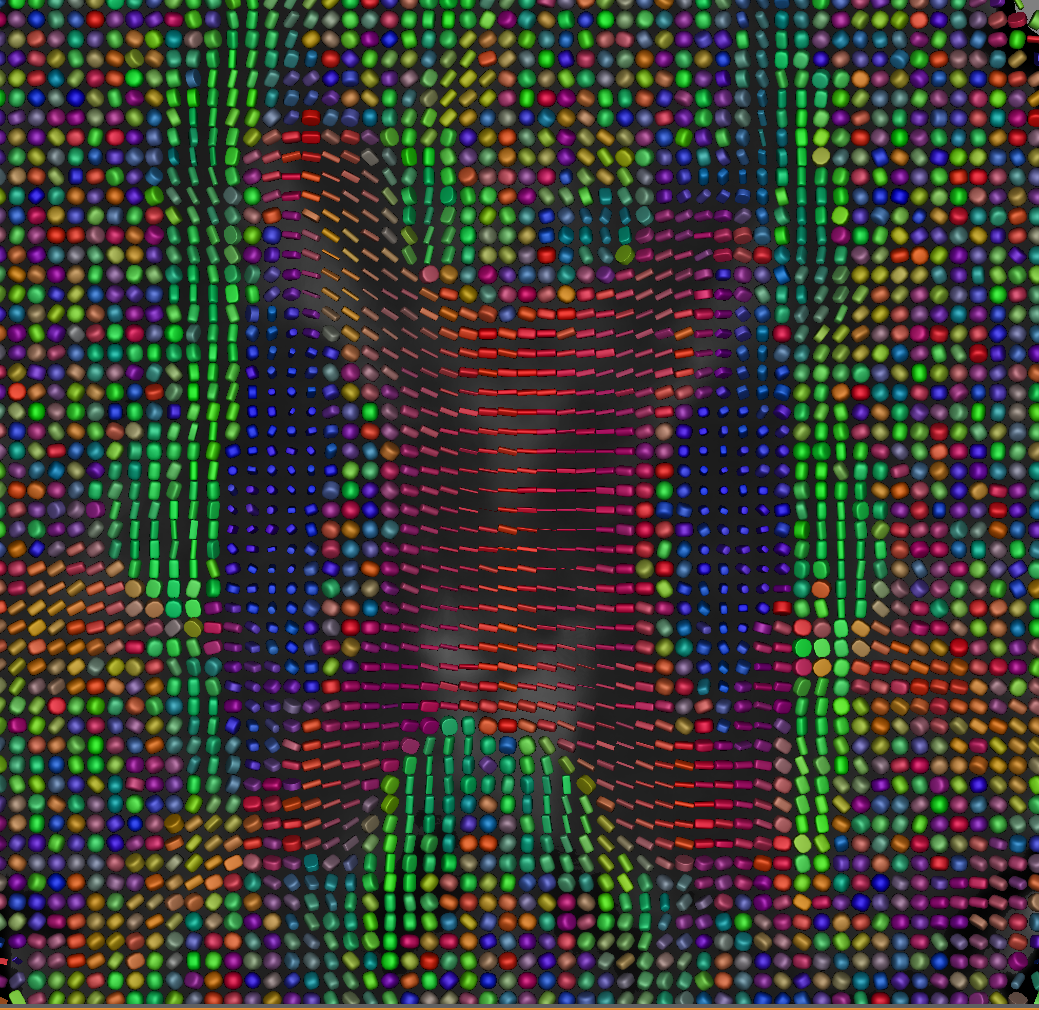
\includegraphics[width=.52\linewidth, angle=0]{figs/Introducao/ex_DTI_Superquadrica.png}
    \label{fig::intro_ex_DTI_glifos}}
    \hfill
    \subfloat[Trato fascículo inferior fronto-occipital (IFOF). A cor predominantemente verde indica sua trajetória, que ocorre na direção anterior-posterior. As linhas são reconstruídas com base no proposto por \citeonline{Weinstein1999} ]{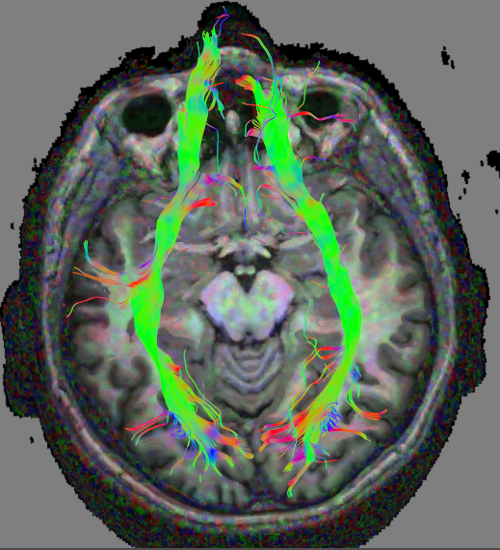
\includegraphics[width=.46\linewidth, angle=0]{figs/Introducao/ex_DTI_tractography.png}
    \label{fig::intro_ex_DTI_tractografia}}
    \hfill
    \label{fig::intro_ex_DTI}
\end{figure}

%\begin{figure}[ht]
%
%\centering
%\includegraphics[width=.485\linewidth, %angle=00]{figs/Introducao/ex_DTI_Superquadric%a.png}
%\centering
%\caption{Tensor de difusão representado por %glifos superquádricos em uma fatia axial do %cérebro na região do corpo caloso. As cores %representam a direção predominante de difusão %onde vermelho é esquerda-direita, azul é %superior-inferior e verde é %anterior-posterior}
%\label{fig::intro_ex_DTI_Superquadrica}
%\end{figure}

%\begin{figure}[ht]
%\centering
%\includegraphics[width=.485\linewidth, %angle=00]{figs/Introducao/ex_DTI_tractography%.png}
%\caption{Trato fascículo inferior %fronto-occipital (IFOF). A cor %predominantemente verde indica sua %trajetória, que ocorre na direção %anterior-posterior}
%\label{fig::intro_ex_DTI_Tractografia}
%\hfill
%\end{figure}

Em tractografia, devido a sua natureza de modelagem, o DTI apresenta limitações. O modelo gaussiano usado no DTI descreve bem regiões de fibras em que o comportamento de difusão ocorre predominantemente em uma direção. Em pontos que contém múltiplas fibras e que estão dispostas nas mais variadas configurações (por exemplo: cruzamento, bifurcação, mistura, "beijo") o modelo gaussiano não sintetiza de forma correta o comportamento da difusão, impedindo o cômputo das direções plausíveis para reconstrução de uma fibra de interesse \cite{fillard2011, daducci2014}. Há um estimativa que entre 66\% a 90\% da substância branca do cérebro contém múltiplas configurações de cruzamento de fibra \cite{descoteaux2015} e a limitação do DTI é um obstáculo para traçar o caminho de fibras do cérebro de forma efetiva.


%\section{Motivação}
%\label{ssec:motivation}

Cientes das limitações do DTI, pesquisadores da área passaram a propor modelos matemáticos mais descritivos do processo de difusão, bem como aplicar estes modelos a volumes de alta resolução angular  (HARDI - \textit{High Angular Resolution Diffusion Imaging}). A tese de doutorado de David Tuch \cite{tuch2002} é o trabalho seminal da área.

Uma aquisição DWI é considerada HARDI se há 45 ou mais gradientes de ponderação de difusão. Esta modalidade de aquisição se diferencia de uma aquisição DTI, que costuma possuir entre 6 a 32 direções \cite{descoteaux2015}.


%\todo{\url{https://www.researchgate.net/figure/Sampling-schemes-in-q-space-a-Cartesian-sampling-dedicated-to-diffusion-spectrum_fig3_319558026}}.
Para aquisições HARDI, foram propostos métodos de imageamento mais descritivos do processo de difusão que o DTI. Alguns deles consistem na abordagem multi-tensor \cite{tuch2002}, o \textit{Q-Ball Imaging} (QBI) \cite{tuch2002, Kindlmann2004}, \textit{constrained spherical deconvolution} (CSD) \cite{tournier2007}, \textit{diffusion spectrum imaging} (DSI) \cite{tuch2002,wedeen2005} e a amostragem generalizada do espaço Q (GQI - \textit{generalized Q-space sampling}) \cite{yeh2010}. Os métodos consistem no cômputo de uma função de distribuição de orientação (ODF - \textit{orientation distribution function}), no qual padrões de fibras subjacentes podem ser inferidos. Para diferenciá-los do DTI, neste trabalho chamaremos estes métodos de imageamento de \textbf{métodos HARDI}.

Uma ODF, no contexto de DWI, consiste em uma função que associa um conjunto de direções a um valor escalar de difusividade. A representação em forma de glifos para ODFs geralmente consistem na plotagem polar esférica (\textit{spherical polar plot}) de uma ODF min-max normalizada no intervalo [0, 1] \cite{TuchQBall2004}, conforme mostrado na Fig. \ref{fig::ex_glifo_hardi}. Chamaremos esta categoria de glifos neste trabalho de \textbf{glifos ODF}. A renderização interativa desses glifos é um ponto principal deste trabalho e os trabalhos de \citeonline{shattuck2008} e \citeonline{peeters2009, almsick2011} trazem diferentes abordagens para este fim.

\begin{figure}[h]
   \centering
       \addtolength{\leftskip} {-2cm} % increase (absolute) value if needed
    \addtolength{\rightskip}{-2cm}

    %\vspace*{3mm}
    \centering
    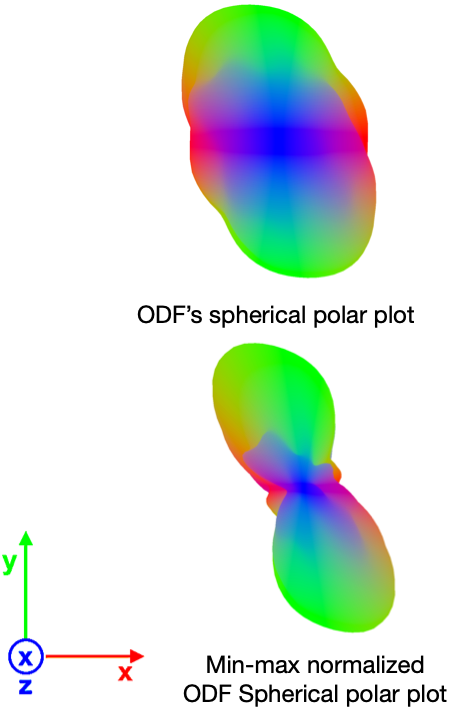
\includegraphics[width=.35\linewidth, angle=0]{figs/Introducao/SphericalMeshModulation.png}
    \caption{Plotagem polar esférica de uma ODF e sua versão min-max normalizada. A normalização enfatiza a direção dominante de difusão. As cores representam a direção no espaço da superfície, onde o vermelho representa horizontal; verde, a vertical; e azul a direção normal ao plano da tela.}
    \label{fig::ex_glifo_hardi}
\end{figure}


A partir de volumes com mais alta resolução angular e métodos HARDI, é possível gerar algoritmos de tractografia melhores e que levem em consideração mais nuances do sinal de difusão que o DTI, especialmente em regiões que contém as mais diversas configurações de múltiplas de fibras. A partir das ODFs, a direção local de fibras em um \textit{voxel} é modelada de forma adequada pela extração de seus máximos locais \cite{fillard2011}, sendo assim a base para algoritmos de tractografia. Porém, aquisições e métodos HARDI não são popularmente utilizadas clinicamente. %\textcolor{red}{Porém, (comentar o que falta ainda para popularizar o seu uso clínico em relação a DTI) ...}

No uso clínico, o DTI é ainda muito mais utilizado que métodos HARDI \cite{descoteaux2015}. As vantagens do DTI se referem a sua aquisição, que requer menos tempo para ser feita e a popularidade de aplicativos que processam DWI por este método de imageamento. Adicionalmente, O DTI demanda uma menor quantidade memória para armazenar parâmetros intrínsecos ao seu método comparados aos métodos HARDI e, geralmente o cômputo de parâmetros relacionados em diferentes aplicações, como o próprio cômputo do método, renderização de glifos e tractografia, são computacionalmente menos exigentes.

%Falar de tratos que HARDI resolve e DTI não?

Em tractografia, tanto baseada em DTI, quanto HARDI, há avanços no entendimento de patologias, como esclerose múltipla, mal de Parkinson, esquizofrenia e derrame \cite{SCHILLING2019194}, e mesmo com essas aplicabilidades, há muitos desafios na área.

Embora os máximos de ODF obtidas através de métodos HARDI consigam resolver os problemas que dizem respeito à estimativa de direções de fibras de forma local, os métodos não inferem sobre a configuração de fibras -- por exemplo, se as diferentes fibras se cruzam ou se "beijam" \cite{SCHILLING2019194}. A busca por informações adicionais para inferir a natureza da configuração entre múltiplas fibras em diferentes regiões é uma oportunidade ainda em aberto.

%%RELER O ARTIGO DO SCHILING E MOSTRAR OPORTUNIDADES 



\todo[inline]{Sugiro mencionar aqui o artigo de Schilling et al. mostrando os desafios ainda em aberto.}

\section{Motivação}
\label{ssec:motivation}

Nosso grupo de pesquisa tem a intenção de fazer um ambiente exploratório para volumes de difusão para volumes de difusão através de um método HARDI. Neste ambiente, um especialista tem total liberdade para construção e análise de forma não invasiva de fibras e para este fim, desenvolveremos um sistema de visualização interativa de perfis de difusão gerados pelo método de imageamento utilizado em glifos e um algoritmo de tractografia interativo, como ilustrado na fluxograma da Fig. \ref{fig::flowchart_vmtk_hardi}.

Diante destes desafios em aberto, este trabalho aborda a implementação de uma método HARDI para processamento de volumes de difusão e a proposição de um algoritmo para renderização interativa de glifos ODF para dados de difusão HARDI. Este algoritmo é integrado ao ambiente de visualização multimodal desenvolvido por \citeonline{voltoline2021}.

%O sistema tem a intenção de ser usado por um especialista para que a partir de um DWI, ele possa construir e analisar de forma não invasiva fibras dos cérebros a partir de um método. Para este fim, 

A visualização interativa de perfis de difusão em cada amostra dá ao especialista uma visão de como o método utilizado o reconstrói a partir do sinal de difusão. A partir dele, pode-se inferir visualmente sobre o método de imageamento utilizado quanto a sua adequabilidade para com a aquisição utilizada. Adicionalmente, há evidências que o uso de glifos superquádricos posicionados em seus respectivos \textit{voxels} em um ambiente de exploração interativa pode melhorar o processo de escolha de parâmetros iniciais em tractografia \cite{voltoline2021}, o que também pode ser aplicado em glifos ODF, visto que, esta categoria de glifos permite o usuário ter a informação de cruzamento de fibras, que não é presente nos superquádricos.

%Acerca do algoritmo de tractografia, a interação com um especialista é relevante nos seguintes aspectos: queremos que o usuário tenha a liberdade de escolher os tratos a serem analisados e que ele possa inferir e assegurar a plausabilidade das conexões das amostras de múltiplas orientações que métodos HARDI proveem.

%Acerca da natureza do tipo de interatividade que queremos mostrar, evidentemente que somente informações extraídas de um volume de difusão não assegura a plausabilidade de fibras reconstruídas e é desejável que haja ferramentas de interatividade para com um especialista para que ele possa escolher regiões de análise e verificar a plausabilidade de fibras.

%O conhecimento de tratos a partir de DWIs é escasso e há discrepâncias entre especialistas, não apenas na área de difusão, mas também na literatura anatômica \cite{SCHILLING2019194} e é necessária a análise humana para inferir sobre a plausabilidade do que está sendo reconstruído.

\begin{figure}[h]
   \centering
       \addtolength{\leftskip} {-2cm} % increase (absolute) value if needed
    \addtolength{\rightskip}{-2cm}

    %\vspace*{3mm}
    \centering
    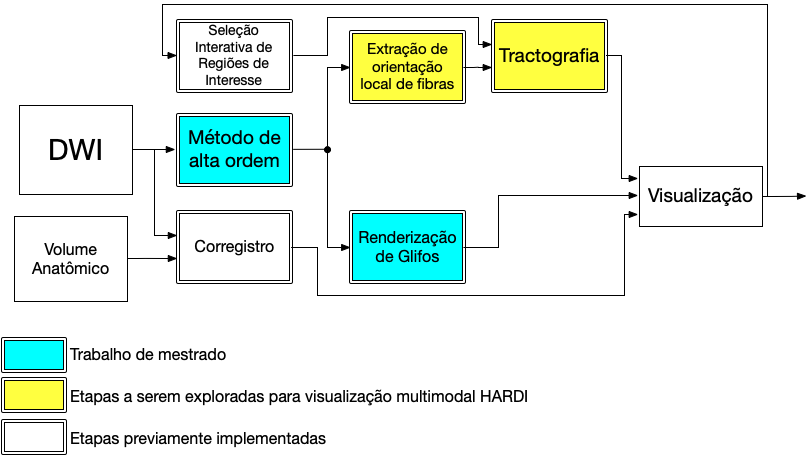
\includegraphics[width=.9\linewidth, angle=0]{figs/Introducao/fluxograma_VMTK_HARDI.png}
    \caption{Fluxograma do ambiente de visualização multimodal HARDI. Os capítulos \ref{chapter::metodos_hardi} e \ref{chap::renderizacao_de_perfis_de_difusao} trazem o detalhamento dos blocos destacados em azul.}
    \label{fig::flowchart_vmtk_hardi}
\end{figure}




%\todo[inline]{Principal motivação é aprimorar a interatividade no processo de reconstrução de uma fibra? Diante dos desafios ainda em aberto, espera-se que, através de uma visualização interativa dos dados de difusão HARDI devidamente pré-processados, um especialista junto com uma máquina construa de forma mais fiel possível, e não-invasiva, as fibras dos tratos (conhecidos e desconhecidos)?}

%\textcolor{red}{No que diz respeito ao método de síntese de orientações das fibras a partir dos volumes HARDI, integramos a sua formulação matemática diretamente no VMTK-Neuro. Os principais critérios para sua escolha se devem a sua adequabilidade em tractografia, sua aplicabilidade em DWIs de baixa resolução angular e simplicidade em relação a quais métodos???.}

%\todo[inline]{Dentre o estado-da-arte da tecnologia HARDI, qual aspecto te chamou atenção e te motivou a desenvolver este trabalho de Mestrado com o objetivo de "implementar e validar um algoritmo (melhor?) de tractografia baseada na técnica de imageamento HARDI"? Na forma como está colocada a sua proposta leva o leitor questionar se o trabalho é simplesmente um exercício do que já se tem.}

%\textcolor{red}{O conhecimento sobre tratos é ainda precário para reconstruí-los integral e automaticamente. É necessária a análise humana para assegurar a plausibilidade das conexões das amostras de múltiplas orientações que a técnica HARDI provê. Para que um especialista possa ter uma visão sucinta e precisa sobre as informações da difusividade local de uma amostra e ajudar uma máquina tomar decisão na ligação desta amostra com as amostras vizinhas para formar uma fibra, é desejável que ele explore de forma interativa tanto os perfis de difusão em cada amostra como as fibras reconstruídas com base nas conjeturas formuladas e reformuladas.}

\section{Ambiente de Implementação}
\label{ssec:ambiente}

Todas as implementações e experimentos do trabalho são realizados no aplicativo VMTK-Neuro (\textit{Visual Manipulation ToolKit for Neuroimages}) \cite{VMTKNeuro}, que é um ambiente de visualização exploratória multimodal multi-plataforma desenvolvida e mantida pelo grupo de pesquisa da Faculdade de Engenharia Elétrica e de Computação da UNICAMP ao qual faço parte. O \textit{software} renderiza em tempo real volumes de ressonância magnética (\textit{magnetic resonance imaging} - MRI) e possui ferramentas de exploração para volumes DWI a partir do DTI. Na subseção \ref{ssec:vmtk-neuro} do capítulo Materiais e Métodos, ilustramos as ferramentas para DWI como um fluxograma e descrevemos as funcionalidades correlatas ao presente trabalho.

% conforme mostrado no fluxograma da figura \ref{fig::PipelineDTI_tracto}.%\textcolor{red}{escaneados com o protocolo Overplus \cite{Philips} e de rastreamento das fibras para volumes DTI sintetizados a partir de DWIs}\todo{não necessariamente Overplus. Overplus não sintetiza as sequencias de aquisições de DWI que há por aí.}.

%\begin{figure}[ht]
%   \centering
%       \addtolength{\leftskip} {-2cm} % increase (absolute) value if needed
%    \addtolength{\rightskip}{-2cm}
%
%    %\vspace*{3mm}
%    \centering
%    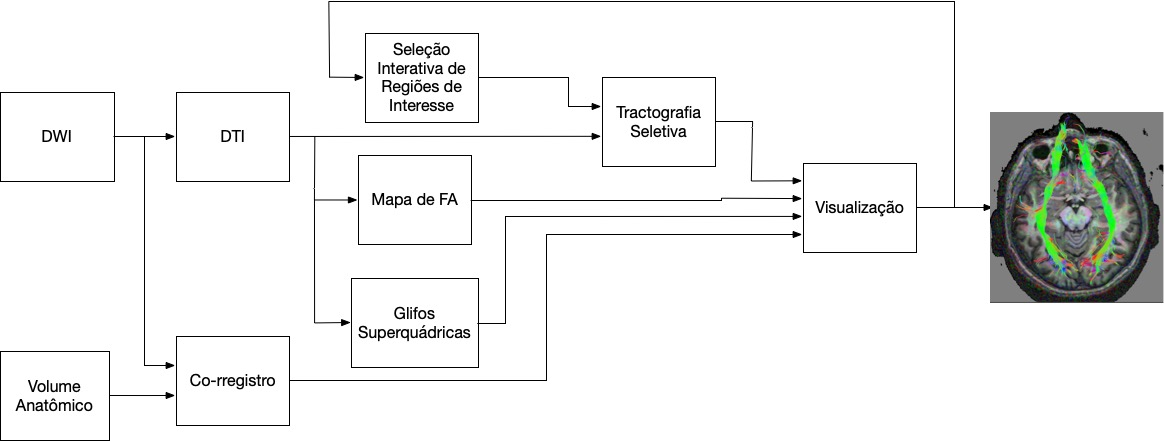
\includegraphics[width=1.0\linewidth, angle=0]{figs/Fluxogramas/PipelineDTI_tracto.jpg}
%    \caption{Fluxograma para tractografia implementado no VMTK-Neuro.}
%    \label{fig::PipelineDTI_tracto}
%\end{figure}

%Estas ferramentas consistem na visualização em tempo interativo de tensores de difusão mapeados em glifos superquádricos \cite{Kindlmann2004} renderizados sobre as suas respectivas amostras (figura \ref{fig::intro_ex_DTI_glifos}), tractografia (figura \ref{fig::intro_ex_DTI_tractografia}) e o corregistro de volumes de difusão com volumes anatômicos T1.

%Na tractografia baseada em DTI, o VMTK-Neuro possui ferramentas de interatividade que possibilitam que o usuário possa inferir sobre as regiões do volume que contém os tratos a serem analisados, bem como filtrar fibras de interesse e eliminar fibras espúrias. Adicionalmente, parâmetros relacionados a reconstrução, que podem diferir de acordo com a região de análise do usuário, também são configuráveis. O algoritmo de tractografia apresenta resultados visuais em tempo interativo para as formas de interação mencionadas.




\section{Objetivos}
\label{sec::objetivos}

A contribuição esperada para o presente trabalho dentro do escopo do ambiente exploratório para DWI através de HARDI é a implementação e validação de um algoritmo de renderização interativo de glifos ODF integrado a um ambiente de visualização exploratória multimodal interativo baseada em um método de imageamento HARDI como um protótipo ao VMTK-Neuro, como ilustrado no fluxograma da Fig. \ref{fig::flowchart_vmtk_hardi}.



A partir do fluxograma, então, é necessário ter de forma esquemática a resposta a questões relativas a:

\begin{itemize}
\item escolha e implementação de um método de imageamento HARDI; %\textcolor{red}{de alta resolução angular (HARDI)}; 
\item visualização interativa de perfis de difusão gerados através do método HARDI;
%\item extração de direções plausíveis de fibras a partir dos perfis de difusão e sua visualização e
%\item implementação de um algoritmo interativo de tractografia .
\end{itemize}


%\textcolor{red}{A expectativa é aplicar os resultados na implementação do fluxograma mostrado na Figura ??? no VMTK-Neuro ...}



%\todo[inline]{Sugiro que mostre em algum ponto uma visão geral do fluxo de controle da sua proposta de construção de tractografia a partir de DWIs de alta resolução angular.}

\section{Desafios}
\label{sec::desafios}

Para implementação do sistema, muito da infraestrutura necessária para alcançar os objetivos estabelecidos estão implementadas no VMTK-Neuro para visualização de volumes DWI por DTI. Portanto, muitos dos desafios enfrentados dizem respeito a questões de implementação do método HARDI e seu esquema de visualização em glifos.

A própria implementação matemática de um método HARDI para sintetizar o perfil de difusão é uma tarefa desafiadora. Os métodos demandam uma quantidade de memória razoavelmente maior que o DTI, que pode ser codificado na memória com apenas 6 elementos (matriz 3x3 simétrica). Métodos HARDI não estabelecem um critério mínimo, entretanto precisam de centenas de elementos para descreverem o perfil de difusão de forma razoável.

A implementação de um esquema de renderização de perfis de difusão em tempo interativo é algo desafiador pela grande quantidade de dados necessários para sintetizar um glifo. Além disso, na renderização tridimensional de volumes de difusão, a renderização de glifos é integrado ao pipeline do próprio esquema de renderização baseada em \textit{raycasting} do volume de ressonância magnética, o que diminui a margem de tempo de execução do esquema para manter a interatividade.

%O último desafio diz respeito à implementação de um algoritmo em tempo interativo de tractografia, que precisa ter seu cômputo rápido o suficiente para seguir as interações feitas pelo usuário.


%\todo[inline]{Não acha que aqui você tem que focar nos desafios relacionados à interatividade, uma vez que o item 4 listado na seção anterior já se encontra implementado no VMTK. Só precisa de algumas adequações. Quais são os desafios para tornar um algoritmo de reconstrução de fibras a partir de HARDI (DWI de alta resolução angular) interativo? Quais restrições devem ser observadas?}

%\sout{No que diz respeito à escolha do método HARDI utilizado, integramos a sua formulação matemática diretamente no VMTK-Neuro. Os principais critérios para sua escolha se devem a sua adequabilidade em tractografia, sua usabilidade em DWIs de baixa resolução angular e simplicidade.}

%\sout{Pela demanda de visualização interativa do VMTK-Neuro, objetivamos que a visualização dos perfis de difusão do método HARDI para os voxels visíveis na tela seja em tempo interativo. Assim, o usuário tem a informação em tempo real dos perfis de difusão nas regiões do volume a serem analisadas.}

%\sout{Assim como a visualização dos perfis de difusão, também objetivamos a visualização interativa da tractografia. As vantagens desta abordagem consistem em dar ao usuário o poder de, através da visualização, escolher regiões de análise e setar os melhores parâmetros de acordo com o seu trato de interesse, indivíduo analisado e aquisição DWI.}

%\section{Contribuições}
%\label{sec::contribuicoes}
%
%
%Este trabalho apresenta duas contribuições:
%
%\begin{itemize}
%	\item proposição de um algoritmo para visualização em tempo %interativo de perfis de difusão para métodos HARDI e
%	\item proposição e validação de um algoritmo de tractografia %em tempo interativo baseado em informações direcionais de %fibras.
%\end{itemize}


%O trato corticoespinhal (CST) (Figura \ref{fig::CST_anatomia}) será o ponto de partida de análise e um ponto central para validação do algoritmo para o escopo deste trabalho de mestrado.

\section{Organização}
\label{sec:intro_organizacao}

O trabalho está organizado em seis capítulos

Como penso em fazer:
Obs: Trabalhos relacionados integrados a cada capítulo.

1)Implementação do método HARDI e extração de fibras subjacentes através de picos.

2) Glifos;

3) Tractografia;

4) Conclusões

\chapter{Materiais e Métodos}

\section{Materiais}






\subsection{VMTK-Neuro}
\label{ssec:vmtk-neuro}

O VMTK-Neuro é um \textit{software} que renderiza em tempo real volumes de ressonância magnética (\textit{magnetic resonance imaging} - MRI) e possui ferramentas de exploração para volumes DWI a partir do DTI, conforme mostrado no fluxograma da figura \ref{fig::PipelineDTI_tracto}. O software utiliza a linguagem de programação em C++ e o OpenGL como API gráfica.

\begin{figure}[ht]
   \centering
       \addtolength{\leftskip} {-2cm} % increase (absolute) value if needed
    \addtolength{\rightskip}{-2cm}

    %\vspace*{3mm}
    \centering
    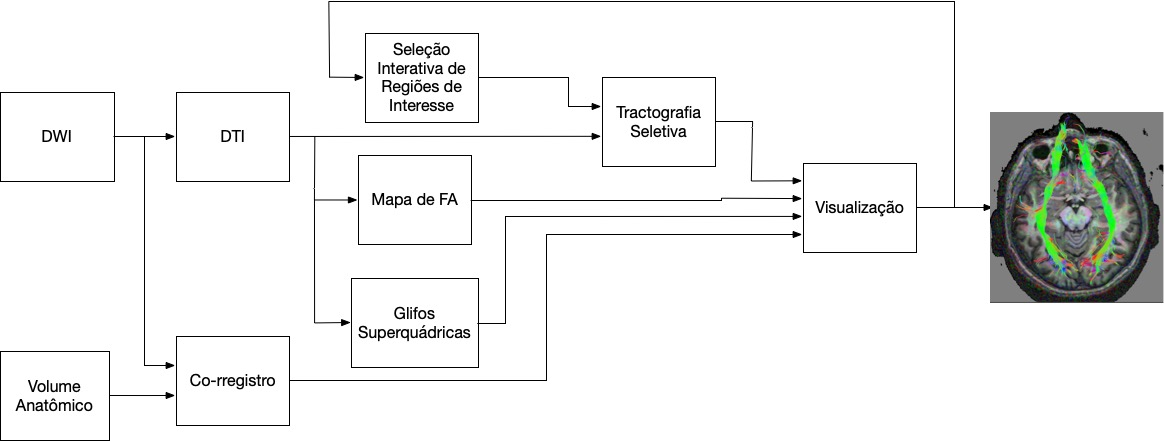
\includegraphics[width=1.0\linewidth, angle=0]{figs/Fluxogramas/PipelineDTI_tracto.jpg}
    \caption{Fluxograma para tractografia e glifos implementado no VMTK-Neuro.}
    \label{fig::PipelineDTI_tracto}
\end{figure}

Estas ferramentas consistem na visualização em tempo interativo de tensores de difusão mapeados em glifos superquádricos \cite{Kindlmann2004} renderizados sobre as suas respectivas amostras (figura \ref{fig::intro_ex_DTI_glifos}), tractografia (figura \ref{fig::intro_ex_DTI_tractografia}) e o corregistro \cite{ting2014} de volumes de difusão com volumes anatômicos T1 .



Na tractografia baseada em DTI, o VMTK-Neuro possui ferramentas de interatividade que possibilitam que o usuário possa inferir sobre as regiões do volume que contém os tratos a serem analisados, bem como filtrar fibras de interesse e eliminar fibras espúrias. Adicionalmente, parâmetros relacionados a reconstrução, que podem diferir de acordo com a região de análise do usuário, também são configuráveis. O algoritmo de tractografia apresenta resultados visuais em tempo interativo para as formas de interação mencionadas.


\subsection{Volumes}

%%%%%VOLUMES UTILIZADOS NOS EXPERIMENTOS


%Temos a intenção de fazer a investigação com dados reais de pacientes do Hospital das Clínicas da UNICAMP, cujo uso foi aprovado pelo comitê de ética CAAE 0893.0.146-000.09, 


No decorrer do trabalho tínhamos a intenção de usar o volumes do bancos de dados do Hospital das Clínicas da UNICAMP, porém os resultados preliminares em termos de conjuntos de ODFs obtidos não se mostraram adequados, e descartamos o uso. Fizemos um estudo para diagnosticar a natureza do problema, que está detalhado na subseção \ref{ssec::problema_overplus} do apêndice, e concluímos que está relacionado ao conjunto de gradientes de ponderação de difusão utilizado no padrão \textit{Overplus}.

Neste trabalho, não pudemos


\section{Métodos}
\subsection{Interatividade}

Pela demanda de visualização interativa do VMTK-Neuro, objetivamos que a visualização dos perfis de difusão de glifos ODF para as amostras visíveis na tela aconteça em tempo interativo. Sendo assim, documentaremos os \textit{benchmarks} de ambos sistemas para atestar o cumprimento deste objetivo.

%\subsection{Tractografia}

%A motivação principal desde trabalho nasceu da seguinte pergunta: "como podemos melhorar a tractografia baseada em DTI do VMTK-Neuro?". Neste contexto, iremos comparar a tractografia baseada em DTI implementada no VMTK-Neuro e a tractografia baseada em HARDI em tratos que há a documentação de falhas do DTI e que são resolvidos pela abordagem que utiliza métodos HARDI.





%\textcolor{red}{
\chapter{HARDI}
\label{chapter::metodos_hardi}
%}

Neste capítulo iremos descrever uma introdução e motivação de métodos HARDI, o método escolhido para sua implementação, bem como os detalhes computacionais de sua implementação.

Este capítulo é a base para as discussões dos capítulos \ref{chap::renderizacao_de_perfis_de_difusao}, em que detalhamos um esquema de renderização para visualização dos perfis de difusão obtidos através destes métodos de imageamento.

\section{Métodos HARDI}
\todo[inline]{Sugiro que façs aqui uma espécie de survey dos métodos ... Fica a seu critério a classificação ... pode ser por forma de amostragem como em \url{https://www.researchgate.net/publication/319558026_High_Angular_Resolution_Diffusion_Imaging_HARDI/link/59e88db8a6fdccfe7f8e8a4f/download} ... Sugiro que poderia fazer um merge com capítulo 3.}

Devido as limitações do DTI para inferir sobre a matéria branca do cérebro, houve uma agenda de pesquisa no início da década de 2000 para de proposição de métodos de imageamento para difusão, e aplicá-los a volumes de mais alta resolução angular. Houveram mais de cem artigos que propuseram métodos de imageamento para descrever o perfil de difusão entre 2000-2010 \cite{descoteaux2015}.

Estes métodos geram uma ODF a partir do sinal de difusão. Geralmente ODFs não possui a restrição quanto a regressão uma função tridimensional que o DTI possui e portanto conseguem ser mais descritivos do processo de difusão e gerar boas aproximações das fibras subjacentes, especialmente em cruzamentos \cite{daducci2014}.

% e evidentemente precisamos fazer uma seleção dos quais deles são mais relevantes para o nosso trabalho.

Os primeiros métodos HARDI propostos consistem no DSI \cite{wedeen2005} - proposto originalmente em 2000 - e presente na tese de doutorado de \citeonline{tuch2002}, juntamente com a abordagem multitensor e o QBI - este último que tem sido o mais popular e está também descrito em artigo \cite{TuchQBall2004}.

Há diferentes aplicativos livres que utilizam métodos HARDI para processamento de DWI, que estão ligados a grupos de pesquisa na área, nos quais restringimos o nosso horizonte a eles. Estes métodos são: GQI (DSI-Studio\footnote{Disponível em: http://dsi-studio.labsolver.org}), QBI (FSL\footnote{Disponível em: https://fsl.fmrib.ox.ac.uk/fsl/fslwiki/FSL}, FiberNavigator\footnote{Disponível em: https://scilus.github.io/fibernavigator/}), CSD (MRTrix\footnote{Disponível em: https://www.mrtrix.org/}).

Para implementação no VMTK-Neuro, o GQI foi escolhido por possuir as seguintes características:

\begin{enumerate}
    \item Ser aplicável em categorias de aquisição com múltiplos valores $b$;
    \item boa aplicabilidade em volumes de mais baixa resolução angular \cite{yeh2010};
    \item ter parâmetros de regularização e filtragem integrados ao método, o que é necessário para detecção da distribuição de fibras adjacentes.
\end{enumerate}

Um ponto importante no processo de decisão é referente a adequabilidade em tractografia. Segundo \citeonline{daducci2014}, não há métodos que se sobressaem em relação a outros nas mais diferentes condições experimentais.

A grande desvantagem do GQI implementado na forma proposta por \citeonline{yeh2010} ocorre no uso de memória. A codificação de ODFs é feita por amostras e requer uma grande quantidade de memória, usualmente nas centenas de números por voxel.

\section{Amostragem Generalizada no Espaço Q}

O método GQI é um modelo livre, derivado da relação de Fourier entre o sinal de difusão e o deslocamento dos spins devido à difusão.

Uma SDF é formada pela soma de várias SDF bases oferecidos por um esquema de amostragem. A relação entre o sinal de difusão é dada pela expressão e a função:

\begin{equation}
    \psi_m(\mathbf{r}, \mathbf{\hat{u}}) = A_qL_{\Delta}\sum_{\mathbf{q}}W(\mathbf{r}, \mathbf{u})sinc(\sigma \sqrt{6D. b(\mathbf{q})}\frac{\mathbf{q}}{|\mathbf{q}|}.\mathbf{\hat{u}})
\end{equation}

onde $W(\mathbf{r}, \mathbf{u})$ é o sinal de difusão no \textit{voxel} de coordenadas $\mathbf{r}$ para uma direção $\mathbf{\hat{u}}$.

A implementação do GQI requer a escolha de um domínio com $n$ direções de difusão de interesse, dadas por $\textbf{U}= \{ \textbf{u}_1, \textbf{u}_2, \textbf{u}_3 ... \textbf{u}_n\}$ em que queremos reconstruir um vetor ODF, dado por $\boldsymbol{\psi} = \{ \psi(\mathbf{u}_1), \psi(\mathbf{u}_2), \psi(\mathbf{u}_3) ... \psi(\mathbf{u}_n)\}$, para cada \textit{voxel} de um volume DWI que tem um conjunto de sinais de difusão $\boldsymbol{e} = \{ W(\mathbf{q}_1), W(\mathbf{q}_2), W(\mathbf{q}_3) ... W(\mathbf{q}_m)\}$ adquiridos sob o conjunto de gradientes $\{\textbf{Q} \}= \{ \textbf{q}_1, \textbf{q}_2, \textbf{q}_3 ... \textbf{q}_m\}$ e valores.

Assim, o método GQI para o cômputo da SDF é através da Eq. \ref{eq::gqi_vec}.

\begin{equation}
    \mathbb{\psi}_m(\mathbf{r}) = \mathbf{S}*\mathbf{E}(\mathbf{r})
\end{equation}

onde S é a matriz de transformação do sinal DWI para amostras de SDF no qual $s_{i,j}$ é dado por:

\begin{equation}
s_{i,j} = sinc(\sigma \sqrt{6D.b(\mathbf{q})}\frac{\mathbf{q}_j}{|\mathbf{q}_j|}.\mathbf{\hat{u}_i}
\end{equation}


Aproximamos a função de orientação de distribuição de difusão pela normalização min-max do vetor de SDF $\mathbf{\psi}(\textbf{r})$, que dá ênfase a informação direcional.


Escolhemos os conjunto $\textbf{U}$ baseado nas malhas esféricas obtidas através de subdivisões do icosaedro. Esta categoria de malha é amplamente utilizada pela comunidade HARDI. Além de \citeonline{yeh2010}, \citeonline{TuchQBall2004} os utilizam em seus respectivos experimentos para ilustrar as suas respectivas ODF. Adicionalmente, \citeonline{descoteaux2007} usa esta categoria de malha para computar a distribuição de fibras adjacentes do QBI em seu respectivo algoritmo de tractografia e isto se deve ao relativo balanceamento dos pontos da malha !!REFERENCIA AQUI e estão ilustrados na Fig. \ref{fig::icosphere}. O conjunto $\textbf{U}$ é obtido através das direções dos vetores normais de cada um dos vértices da malha.

Neste trabalho, nos restringimos a categoria de malhas feitas através das subdivisões de ordem $2^k$ do icosaedro.

\begin{figure}[ht]
\centering
\captionsetup[subfloat]{farskip=0pt,nearskip=0pt}
\centering
    \subfloat[Tesselação de $2^a$ ordem] {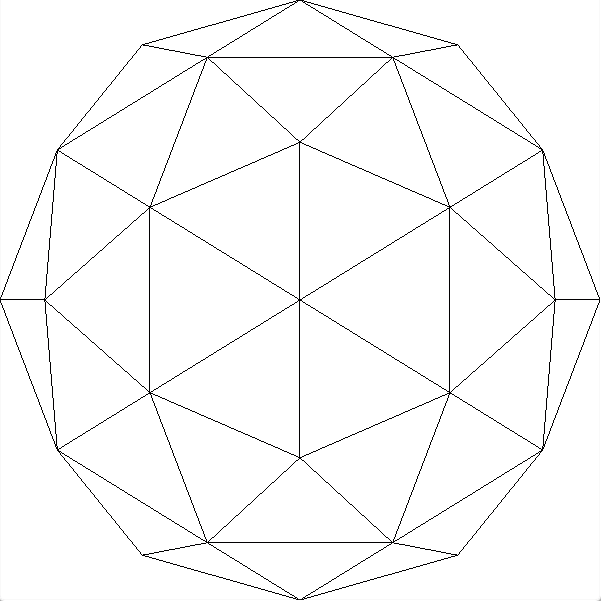
\includegraphics[width=.25\linewidth, angle=0]{figs/HARDI/Icosphere/icosphere_1.png}
    \label{fig::icosphere_1}
    }
    \hspace{1em}
    \subfloat[Tesselação de $4^a$ ordem] {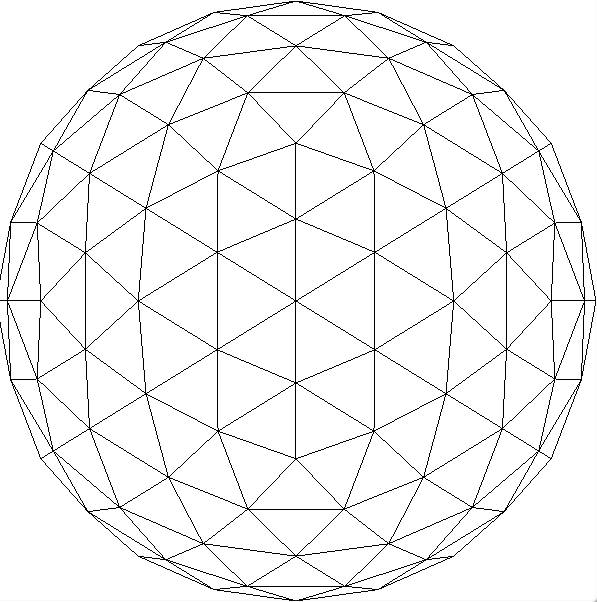
\includegraphics[width=.25\linewidth, angle=0]{figs/HARDI/Icosphere/icosphere_2.png}
    \label{fig::icosphere_2}
    }
    \\
    \subfloat[Tesselação de $8^a$ ordem] {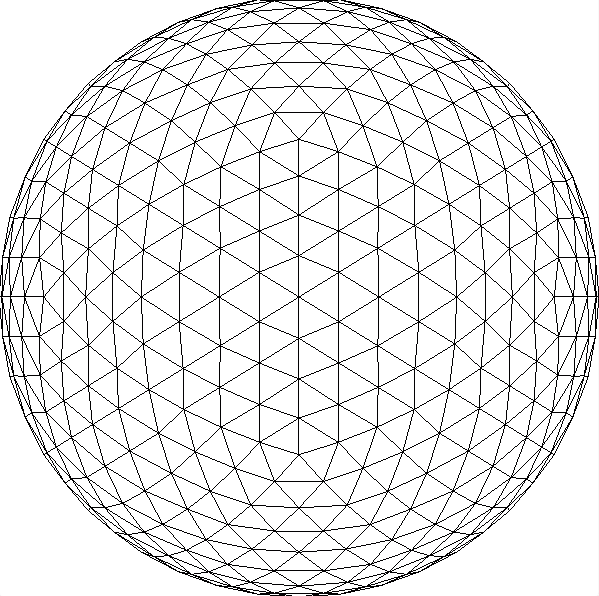
\includegraphics[width=.25\linewidth, angle=0]{figs/HARDI/Icosphere/icosphere_3.png}
    \label{fig::icosphere_3}
    }
    \hspace{1em}
    \subfloat[Tesselação de $16^a$ ordem]{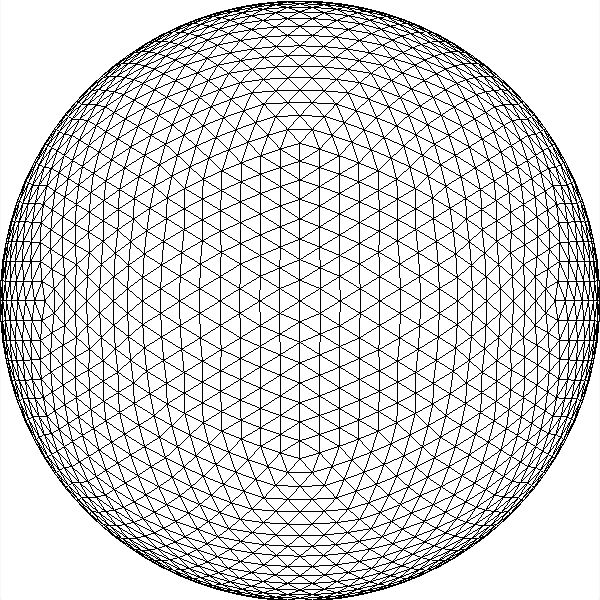
\includegraphics[width=.25\linewidth, angle=0]{figs/HARDI/Icosphere/icosphere_4.png}
    \label{fig::icosphere_4}
    }
     \caption{Esferas obtidas através da tesselação de um icosaedro.}
    \label{fig::icosphere}
\end{figure}

A quantidade de amostras em função da ordem de tesselação do icosaedro é dada por:

\begin{equation}
    N = 10\times t^2 + 2
\end{equation}

onde $t$ é a ordem de tesselação. A respeito das malhas esféricas mostradas na Fig. \ref{fig::icosphere}, a quantidade de vértices para $2^a$, $4^a$, $8^a$ e $16^a$ ordem de tesselação é 42, 162, 642 e 2562, respectivamente.


Devido a simetria das ODFs em relação aos eixos x, y, z, onde $R(\textbf{u}) = R(-\textbf{u})$, implementamos o cômputo das ODFs na metade da esfera, o que permite que a quantidade de dados por \textit{voxel} seja diminuída pela metade.

Pode-se estabelecer que a estrutura de dados de $\mathbf{U}$ seja $[\mathbf{u_1}, \mathbf{u_2}, ..., \mathbf{u_{N-1}}, \mathbf{u_{N}}]^T$. Porém, podemos aproveitar a simetria dos dados e da malha esférica utilizada e organizarmos os dados de tal forma que 




\chapter{Renderização de perfis de difusão}
\label{chap::renderizacao_de_perfis_de_difusao}

\todo[inline]{Falta contextualizar nos objetivos que você listou na seção 1.3. Não é melhor focar em renderização de perfis de difusão que é um dos problemas relacionados diretamente com a interatividade?}

Neste capítulo, apresentamos uma abordagem de um esquema de renderização interativa de múltiplas ODFs através de sua plotagem polar esférica, a sua integração ao VMTK-Neuro, resultados visuais e o seu \textit{benchmark}, mostrado através do FPS (\textit{frames} por segundo) em função da quantidade de glifo.

\todo[inline]{Eu deixaria o parágrafo abaixo para conclusões}
Ressaltamos que o esquema de renderização de perfis de difusão pode ser utilizado por outros métodos de imageamento de difusão e para outras funções esféricas que sejam representadas através conjunto de amostras.

%Esta classe de glifos são amplamente utilizados como uma ferramenta de visualização para prova de conceito em trabalhos na área de DWI. Além de \citeonline{TuchQBall2004}, alguns trabalhos relacionados que os utilizam são: \citeonline{SCHILLING2019194}, para ilustrar a eficácia de métodos HARDI na detecção de direções de difusão, \citeonline{descoteaux2007}, para mostrar o efeito de uma técnica pré-processamento proposto em ODFs que melhora a tractografia e \citeonline{yeh2010} os utilizam como ferramenta de visualização para o método de imageamento proposto em seu trabalho.

%\section{Cômputo de funções de distribuição de orientação de difusão}

%Foi aplicado o algoritmo proposto por \citeonline{TuchQBall2004}\sout{, que}\textcolor{red}{Este} consiste na discretização da FRT para amostras contida num domínio esférico discreto $\{\textbf{u}\}$. O domínio $\{\textbf{u}\}$ utilizado é proveniente de uma malha esférica gerada a partir de subdivisões de um icosaedro, conforme representado na figura \ref{fig::MalhaEsferico}.
%\textcolor{red}{Esta subdivisão proporciona uma distribuição mais uniforme dos pontos em comparação com os pontos gerados pela parametrização em coordenadas esféricas $(\phi, \theta)$ \cite{TuchQBall2004, descoteaux2007_QBI, yeh2010}}.

%Um exemplo de malha esférica obtida com essa abordagem está ilustrado na figura \ref{fig::MalhaEsferico}.


%\begin{figure}[ht]

%\subfigcapskip = -5pt
%    \centering
    %\vspace*{1mm}
   % \includegraphics[width=0.4\linewidth, angle=0]{figs/Exemplos_QBall_visualizacao/Mesh%EsfericoIco.png}
 %       \caption{Malha Esférica a partir de duas subdivisões de um icosaedro. Esta malha possui 162 vértices não-colineares}
%    \label{fig::MalhaEsferico}
 %   \hspace{1pt}
%\end{figure}

%\todo[inline]{Está confuso. Quem propôs usar icosaedro?}
%\sout{A motivação da escolha desta categoria de malha esférica consiste em uma distribuição mais uniforme dos pontos na esfera em comparação a outras abordagens. Comparando com a malha gerada partir de discretizações nas coordenadas esféricas $(\phi, \theta)$, a distribuição de pontos é mais concentrada de pontos nos polos e mais esparsa no equador. Esta categoria de malha é referenciada em trabalhos da área como base de amostras para descrever funções esféricas \cite{TuchQBall2004, descoteaux2007_QBI, yeh2010}.}

%\todo[inline]{Procure conectar as partes do seu texto. Ligue o "cômputo" com a Equação que você apresentou antes.}

%\sout{A abordagem de implementação consiste no cômputo de todas as ODFs} Para cada \textit{voxel} do DWI\textcolor{red}{, todas as funções de distribuição de orientação (ODFs) foram computadas} para \textcolor{red}{todas} as direções representadas na malha com uso da Equação \ref{???} e \sout{seu armazenamento}\textcolor{red}{foram armazenadas} na memória para posterior uso na tractografia e geração de glifos.


\section{Visualização de funções de distribuição de orientação}

A forma mais comum de visualizar dados derivados de ODFs através de métodos HARDI é através glifos provenientes da plotagem polar esférica.

Estes glifos dão uma visualização clara do comportamento local de difusão e são amplamente utilizados para provas de conceito em trabalhos na área de DWI. Alguns dos exemplos de trabalhos que os utilizam, temos: \citeonline{TuchQBall2004} e \citeonline{yeh2010} os utilizam como ferramenta de visualização para o método de imageamento propostos em seus respectivos trabalhos, \citeonline{daducci2014} os utiliza para ilustrar e comparar ODFs reconstruídas por diferentes métodos, \citeonline{SCHILLING2019194} os usam para ilustrar a eficácia de métodos HARDI na detecção local de direções de fibras subjacentes, \citeonline{descoteaux2007}, para ilustrar transformações entre ODFs no seus respectivos algoritmos de tractografia propostos.

Este esquema de renderização, integrado a um sistema de visualização para DWI pode ser uma ferramenta poderosa para pesquisadores da área para avaliar perfis de difusão locais e melhorar o seu entendimento em métodos HARDI.



%Esta classe de glifos são amplamente utilizados como uma ferramenta de visualização para prova de conceito em trabalhos na área de DWI. Além de \citeonline{TuchQBall2004}, alguns trabalhos relacionadosque os utilizam são: \citeonline{SCHILLING2019194}, para ilustrar a eficácia de métodos HARDI na detecção de direções de difusão, \citeonline{descoteaux2007}, para ilustrar o efeito de um\sout{a técnica} \todo{qual pré-processamento?}pré-processamento \sout{proposto} em ODFs que melhora a tractografia e \citeonline{yeh2010} 

%Foi implementado um esquema de visualização para ODFs em glifos de acordo através de representações gráficas polares esféricas. A implementação serviu primeiramente para prova de conceito e posteriormente otimizada para que seja possível a sua renderização, \textit{voxel} a \textit{voxel}, em tempo interativo pelo VMTK-Neuro, o que foi possível nos testes feitos em um Macbook Pro Retina 13', com processador Intel Core i5 Dual-Core 2.7Ghz, processador gráfico Intel Iris Graphics 6100 1536 MB e memória RAM de 8 GB 1867 MHz DDR3.

\todo[inline]{Fazer uma breve justificativa da relevância da visualização das ODFs no contexto da sua proposta de uma visualização interativa almejando uma tractografia mais próxima dos tratos reais.}

\subsection{Plotagem polar esférica}

%Como descrito na seção \ref{sec::trabalhos_relacionados_glifos}
A forma do glifo consiste na modulação do raio na direção $\mathbf{u}$ de uma esférica de acordo com uma versão normalizada do seu valor de imagem na função $\psi(\mathbf{u})$. A normalização que fizemos neste trabalho para representação está representado na equação \ref{eq::normglifo2}.

\begin{equation}
\label{eq::normglifo2}
    R(\mathbf{u}) = \frac{\psi(\mathbf{u}) - min(\psi(\mathbf{u}))}{max(\psi(\mathbf{u})) - min(\psi(\mathbf{u}))}
\end{equation}

As cores dos glifos consistem em um mapeamento das coordenadas dos vértices $(x_v,y_v,z_v)$ da malha esférica para as suas componentes RGB de acordo com a equação \ref{eq::cor_glifo} e ilustrado nos glifos da figura \ref{fig::glifo_ilustrado}. Esta forma de mapear, além de simples, entra muito em acordo com a codificação em cores definidos no mapa de FA e faz o entendimento do glifo ser intuitivo. %\todo{É imprescincível adicionar esta informação?}\sout{Não foi implementado o cômputo de vetores normais à superfície representadas pelo glifo, que consequentemente não tem iluminação associada.}

\begin{equation}
\label{eq::cor_glifo}
    (r,g,b) = (|x_v|,|y_v|,|z_v|)
\end{equation}

\begin{figure}[ht]

%\subfigcapskip = -5pt
    \centering
    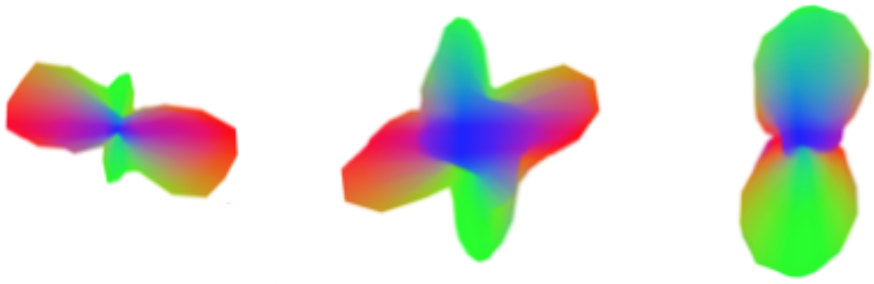
\includegraphics[width=.8\linewidth, angle=0]{figs/Esquema_Glifo/Glifos3Ex.png}
    \caption{Exemplos de glifos rasterizados de perfis de difusão que consistem em uma malha esférica modulada através da equação \ref{eq::normglifo2} e com as cores de acordo com a equação \ref{eq::cor_glifo}}
    \label{fig::glifo_ilustrado}
   \hspace{1pt}
\end{figure}

Neste trabalho, chamaremos a plotagem polar esférica aplicada a ODFs de métodos HARDI de glifos HARDI.

\section{Trabalhos Relacionados}

Apesar da relevância reconhecida da renderização interativa de dados HARDI, a comunidade não tem explorado muito esta questão. Por questões de performance, nos limitaremos a trabalhos que exploram recursos da GPU. Há duas grandes abordagens achadas na literatura para renderização de glifos. A primeira é baseada em \textit{ray-casting}, onde a geometria do glifo é representada por uma função ou expressão algebrica \cite{peeters2009, almsick2011}. A outra é baseada na renderização de malhas, com a geometria do glifo aproximada por malhas poligonais \cite{shattuck2008}.

\citeonline{shattuck2008} tessela uma representação polar de ODF com triângulos, onde a superfície do glifo é gerada através da discretização do seu domínio polar, e sua forma é gerada na CPU através de uma função analítica neste domínio. Os glifos são renderizados por fatia. Com a mudança de malha e parametros de visualização, os vertices do glifo são recomputados e reenviados à GPU. A performance relatada é de dez \textit{frames}/s para uma fatia de um volume, no qual cada glifo tem 225 vertices, em uma cena com aproximadamente 2 milhões de triângulos. Neste trabalho, exploramos recursos da GU modernos para melhorar a performance de renderização e uso de memória da GPU.




\citeonline{peeters2009} apresentaram um esquema de renderização utilizando \textit{ray-casting}. Na CPU, o centro, o raio da esfera delimitadora e o cubo delimitador por glifo são computados. Na GPU, o algoritmo de ray-casting é executdo por pixel no \textit{fragment shader}. Se o raio lançado para um pixel não intercepta a esfera delimitadora, o fragmento é descartador. Caso contrário, o algoritmo executa uma busca linear ,com passos discretos para interseção da ODF para com o raio. Tles alcançaram uma melhor performance que o algoritmo apresentado por \citeonline{shattuck2008}. \citeonline{almsick2011} melhorou a busca por interseção utilizando o método numérico \textit{regula falsi} e cilindros delimitadores alinhados com o eixo de visão. Eles atingiram um melhor tempo de performance sem sacrificar a qualidade de renderização, documentando que 9000 glifos puderam ser gerados a 30 fps. Há um problema crítico na acurácia e eficiência do raio lançado. Quando o raio tende a ser paralelo ao glifo, muitas iterações podem ocorrer em algumas \textit{threads}. A renderização baseada em triângulos que propomos neste trabalho não apresenta este problema. 

\citeonline{voltoline2021} propuseram um esquema de renderização para glifos superquádricos para tensores \cite{Kindlmann2004}. Eles exploraram alguns recursos modernos da GPU para atingir este objetivo, que consistem em \textit{transform feedback}, aproximação triangular adaptativa dos glifos e renderização por instanciação indireta. Diferentemente das superquádricas, os dados associados com glifos ODF são bem maiores, o que inviabiliza sua armazenagem na GPU. Consequentemente, devemos propor estratégias para subdividir a grande quantidade de dados em um conjunto de "tijolos" que cabem na memória da GPU para os glifos a serem renderizados.

\section{Renderização de Glifos ODF}

\subsection{Geometria base}

\subsection{Atributos}

Para renderizarmos $M$ glifos com um comando de desenho, usamos instanciação de GPU. A geometria base selecionada, reference a $2^t$-ésima ordem de tesselagem do icosaedro é instanciada por um vetor de translação e amostras de ODF.

Para $M$ \textit{voxels} visíveis, enviamos os vetores de translação como um atributo por instância, que é computado em função das coordenadas de \textit{voxel} $(v_x, v_y, v_z)$ como:

\begin{align}
 \label{eq::translation}
    dx = (v_x + 0.5).spacing_x \nonumber\\
    dy = (v_y + 0.5).spacing_y \\
    dz = (v_z + 0.5).spacing_z \nonumber
\end{align}

Note que os dados de voxel visíveis retornados pelo algoritmo é armazenado em um buffer na GPU. Este dado é utilizado diretamente no algoritmo de renderização no \textit{vertex shader} para cômputo do atributo de translação.

Como mencionado no capítulo \ref{chapter::metodos_hardi}, aproveitamos a simetria dos dados de ODF para organizarmos os dados no domínio de um hemisfério. Para o voxel de índice $M$, os elementos são organizados como $[R_m(\mathbf{u_1}), R_m(\mathbf{u_3}), ..., R_m(\mathbf{u_{N-3}})$, $R_m(\mathbf{u_{N-1}})]^T$. Onde cada elemento $R_m(\mathbf{u}_{K})$ desloca os pontos $P_{2K-1}$ e seu simétrico $P_{2K}$ no $m$-ésima geometria base instanciada.

Para a geometria base escolhida, geramos uma matriz com os dados de ODF enviados à GPU como a matriz $\mathbf{R}_{\frac{V}{2}xM}$ (Eq. \ref{eq::R}), onde $V$ é o numero de vértices da geometria base, dado por $10 \times 4^t + 2$. As amostras de ODF consistem nos primeiros $V/2$ do vetor de valores de ODF a serem renderizados. Cada coluna $R_m(\mathbf{u})$ refere-se à ODF referente ao $m$-ésimo índice de voxel visível, dado por $d_m$. $\mathbf{R}$ é enviado à GPU como uma textura 2D de formato RGBA.

\begin{equation}
\label{eq::R}
\mathbf{R} = 
\begingroup % keep the change local
\setlength\arraycolsep{2pt}
\begin{bmatrix} 
    R_1(\mathbf{u}_1) &     R_2(\mathbf{u}_1)      & \cdots  &     R_M(\mathbf{u}_{1})  \\    
     R_1(\mathbf{u}_3)&     R_2(\mathbf{u}_3)      & \cdots  &     R_M(\mathbf{u}_{3}) \\
    \vdots & \vdots & \vdots & \vdots  \\    
     R_1(\mathbf{u}_{V-1}) & R_2(\mathbf{u}_{V-1}) & \cdots  & R_M(\mathbf{u}_{V-1})
\end{bmatrix}.
\endgroup
\end{equation}

Cada \textit{texel} no format RGBA suporta quatro valores. Agrupamos os valores escalar $[R_m(\mathbf{u_1}), R_m(\mathbf{u_3}), ..., R_m(\mathbf{u_{V-3}}), R_m(\mathbf{u_{V-1}})]^T$ de quatro em quatro, como mostrado na Fig. \ref{fig::texelfetch}, consequentemente, em cada acesso de \textit{texel}, tenhamos quatro valores escalares $R_j(\mathbf{u_{8K+1}})$ (R), $R_j(\mathbf{u_{8K+3}})$ (G), $R_m(\mathbf{u_{8K+5}})$ (B), $R_m(\mathbf{u_{8K+7}})$ (A). Nos quais deslocamos quatro pares de pontos simétricos na geometria base $P_{8K+1}$, $-P_{8K+1}$, $P_{8K+3}$, $-P_{8K+3}$, $P_{8K+5}$, $-P_{8K+5}$, $P_{8K+7}$, $-P_{8K+7}$ para o j-ésimo glifo visível (também j-ésima instância). Desta forma, as dimensões da textura com dados ODF dos dados de ODF é $ \frac{V/2}{4} \times M$. Se $\frac{V}{2}$ não é divisível por quatro, é necessário inserir mais linhas abaixo da última com valores \textit{dummy}, para que o número de linhas se torne divisível, o que há a certificação de que cada coluna de $\mathbf{R}$ possa ser acessada com o índice de instância.

!!IMAGEM!! TEXELFETCH

Os dados de ODF são acessados no \textit{vertex shader}, quando cada glifo da $j$-ésima instância é processada. Todos os \textit{texels} $K = \lfloor\frac{Vertex\_ID}{8} \rfloor$ na coluna são acessados para pegar um grupo de 4 valores de ODF para deslocar oito pontos. Usamos a função \textit{texelFetch} para acessar diretamente a textura de ODF utilizando coordenadas não-normalizadas $(j, \lfloor\frac{Vertex\_ID}{8} \rfloor)$. O valor utilizado para \textit{lookup} da componente  para deslocar o seu respectivo ponto na geometria base no vertex shader é acessível pela análise do resto da divisão por oito do Vertex\_ID, como ilustrado na Fig. \ref{fig::texelfetch}. Adicionalmente, utilizando a notação via colchetes, onde as componentes R, G, B e A são mapeados nos índices 0, 1, 2 e 3, respectivamente, o escalar de ODF pode ser mapeado por $\lfloor (Vertex\_ID \mod{8})/2 \rfloor$.




%, no qual foi aperfeiçoado por \cite{almsick2011}. Esta abordagem possibilitou incrementos em performance em relação a \citeonline{shattuck2008}.

%\citeonline{raphael_dissertacao} propôs um esquema de renderização interativa do tensor de difusão em glifos superquádricos \cite{Kindlmann2004} utilizando polígonos. Em seu trabalho, os glifos são renderizados a taxas interativas e a sua abordagem consiste na minimização de tráfego de dados entre CPU-GPU, que consiste apenas em parâmetros que customizam e deslocam os glifos, e o uso de renderização por instâncias. Adicionalmente, este esquema está integrado ao VMTK-Neuro. Os resultados obtidos neste trabalho nos influenciou a adaptar o seu esquema para glifos HARDI.



%\subsection{\sout{Abordagem de renderização}}

%\sout{\citeonline{peeters2009} apresentou pela primeira vez um esquema de renderização para esta categoria de glifos, nos quais são aperfeiçoados por \citeonline{almsick2011} e \citeonline{hlawitschka2012}. Estes esquemas utilizam a abordagem \textit{raycasting}.}

%\sout{No VMTK-Neuro, um dos algoritmos de renderização do tensor difusão por glifos superquádricos é feita por instanciações de uma malha esférica, no qual é customizada por parâmetros particulares a cada tensor de difusão referentes a cada \textit{voxel} detectado e posicionado na cena de acordo. Este esquema de renderização desenha os glifos em tempo interativo.}

%\sout{Pela maior simplicidade e boa efetividade da renderização por instanciações de uma malha esférica, o esquema desenvolvido neste trabalho utiliza esta abordagem.}



%Dados relativos ao desempenho \sout{serão mais detalhados na dissertação de mestrado}\textcolor{blue}{estão disponíveis no link ...}.



%\sout{Medições do tempo relativo ao desempenho foram feitas para a quantidade de 197 vértices da malha esférica \sout{em um}\textcolor{blue}{num} volume de resolução 128x128x90. Para uma quantidade na faixa de 5000 glifos renderizados simultaneamente sobre uma fatia completa, obtemos tem um tempo de resposta entre 80 e 110ms. Para uma quantidade pequena de glifos na faixa das dezenas, o tempo de resposta cai para o intervalo entre 60 e 70ms. Esse tempo de resposta está nas proximidades ou é menor do que o tempo de 0,1s, que é o limite máximo para que o usuário tenha a percepção de resposta instantânea da máquina e que suas ações são a causa de que algo aconteça na tela \cite{nielsen1994}.}

%\sout{No cômputo das ODFs do \textit{QBall}, é feito o mapeamento do sinal de DWI para a ODF a partir das direções derivadas da malha esférica. O glifo para visualização é gerado diretamente de acordo a representação gráfica polar esférica em que $R(\textbf{u}) = \psi(\mathbf{u})$, onde \textbf{u} é a direção de difusão. A malha esférica utilizada para geração dos glifos em \ref{section::QBall_Glifos} está representada na figura \ref{fig::MalhaEsferico}.}

%A priori, todas as ODFs são calculadas e normalizadas para o intervalo $[0,1]$ para cada um dos \textit{voxels} do volume e referenciadas no processo de renderização.

%O formato de armazenamento dos valores ODF associados à malha consiste numa lista de valores escalares associados a cada um dos \textit{voxels}.



%\todo[inline]{Falta uma descrição melhor de como são construídos os glifos a partir de ODFs e o seu mapeamento às entidades gráficas. Isso torna difícil o entendimento da sua implementação. !!Descrito em trabalhos relacionados!}
\section{Esquema de renderização de glifos HARDI}

%A abordagem utilizada para renderização consiste em instanciações de uma malha esférica de N vértices centrada na origem e raio unitário, que é enviada à GPU uma única vez e sem repetição de vértices nos seus dados. A cada instância, a malha é transformada por uma matriz de translação e as suas amostras de ODF.

%A matriz de translação posiciona o centro da malha esférica para a sua respectiva posição. O perfil de difusão diz respeito às ODFs particulares a cada glifo, que determina a forma do glifo através da multiplicação do vértice da malha associada à direção de difusão ao seu valor de ODF.

%Estes elementos são enviados da CPU à GPU a cada requisição de desenho que tem como entrada uma lista de matrizes de translação e de amostras de ODF. Então, para atingirmos o objetivo da interatividade, é desejável que o tráfego de dados entre as partes seja o mínimo possível e sem redundância na descrição do objeto.

%O envio do conjunto de coordenadas de translação à GPU consiste no envio de um vetor contendo P matrizes de translação como um atributo, que é único para cada malha esférica instanciada.

%Os dados relativos a ODF enviados para GPU consistem nas N amostras referentes ao perfis de difusão para cada um dos P glifos a serem desenhados. A forma que as amostras de ODF são enviadas à GPU consiste na construção e envio de uma matriz $\mathbf{\Psi}_{PxN}$, onde P é a quantidade de glifos a serem desenhados e N consiste na quantidade de amostras de ODF utilizada. O envio da matriz $\mathbf{\Psi}$ à GPU é feito como uma textura 2D. 

%Na matriz $\mathbf{\Psi}$, o elemento da i-ésima linha na j-ésima coluna da matriz se refere à ODF do i-ésimo glifo a ser desenhado associado ao j-ésimo vértice da esfera, que por sua vez tem as coordenadas da direção $\mathbf{u}_j$. Chamaremos  a ODF na i-ésima linha de $\psi_i(\mathbf{u})$ e o seu valor no j-ésimo vértice da esfera de $\psi_i(\mathbf{u}_j)$.

%A recuperação na GPU das ODFs é feita através dos índices de instância e vértice. Para isto, é necessário que o índice de vértice (\textit{gl\_VertexID}\footnotemark) da direção de cada um dos vértices correspondam à coluna do seu respectivo valor de ODF $\psi(\mathbf{u}_j)$ na matriz de perfis de difusão. O acesso das linhas da matriz de perfis de difusão, correspondentes aos perfis de difusão de um \textit{voxel} é acessível pelo índice de instância (\textit{gl\_InstanceID}\footnotemark[\value{footnote}]). Tendo os dados organizados desta maneira estabelecida, o acesso é feito no \textit{vertex shader} utilizando através da função \textit{texelFetch}\footnotemark[\value{footnote}] com os argumentos de acesso de linha e coluna através do par (\textit{gl\_VertexID}, \textit{gl\_InstanceID})\footnotemark[\value{footnote}]\footnotetext{Todos os comandos foram implementados em OpenGL com a linguagem para \textit{shader} GLSL.}. A forma de acesso na GPU da matriz de perfis é ilustrada na figura \ref{fig::GPU2glifoGeneral}.




%A figura \ref{fig::organizacao2GPU} ilustra \todo{Não entendi ... a organização é dinâmica? Isso é muito custoso!}\textcolor{brown}{a organização dos dados para quando ocorre a detecção de quatro \textit{voxels}}.

%Na GPU, a malha esférica, copiada anteriormente e alocada em um \textit{vertex buffer object} (VBO), é instanciada P vezes. A recuperação na GPU das ODFs é feita através dos índices de instância e vértice. Para isto, é necessário que o índice de vértice (\textit{gl\_VertexID}\footnotemark) da direção de cada um dos vértices correspondam à coluna do seu respectivo valor de ODF $\psi(\mathbf{u})$ da matriz de perfis de difusão. O acesso das linhas da matriz de perfis de difusão, correspondentes aos perfis de difusão de um \textit{voxel}acessível pelo índice de instância (\textit{gl\_InstanceID}\footnotemark[\value{footnote}]). Tendo os dados organizados desta maneira estabelecida, o acesso é feito no \textit{vertex shader} utilizando através da função \textit{texelFetch}\footnotemark[\value{footnote}] com os argumentos de acesso de linha e coluna através do par (\textit{gl\_VertexID}, \textit{gl\_InstanceID})\footnotemark[\value{footnote}]\footnotetext{Todos os comandos foram implementados em OpenGL com a linguagem para \textit{shader} GLSL.}. A forma de acesso na GPU da matriz de perfis é ilustrada na figura \ref{fig::GPU2glifoGeneral}.

%A cor dos glifos é definida de acordo com o vértice da malha esférica instanciada no \textit{vertex shader} e definida de acordo com a equação \ref{eq::cor_glifo}.


%f


O objetivo desta seção é detalhar o esquema de renderização de glifos baseada em polígonos. Na subseção \ref{ssec::initializacao_glifo}, descrevemos a inicialização do esquema; na subseção \ref{ssec::datastruct} detalhamos a estrutura de dados que consistem no tráfego CPU-GPU a cada requisição de renderização; na subseção \ref{ssec::otimizacao}, mostramos uma adaptação da estrutura de dados para ODF simétricas de modo a diminuir o tráfego CPU-GPU; na subseção \ref{sssec::visao_shaders}, esquematizamos as funcionalidades do \textit{vertex} e \textit{fragment shaders}.


A quantidade de amostras $N$ de ODF que customizam os glifos de forma razoável costumam estar na casa das centenas \cite{TuchQBall2004, yeh2010}, o que gera uma grande quantidade de dados enviados à GPU nas requisições de desenho. Assim, os procedimentos sugeridos nas subseções \ref{ssec::datastruct} e \ref{ssec::otimizacao} são fundamentais ao esquema pois consistem em expor estratégias para minimizar ao máximo o tráfego de dados CPU-GPU.


%\todo[inline]{Incluir os pseudocódigos de shaders não ajudaria o entendimento da ideia?}

\subsection{Inicialização}
\label{ssec::initializacao_glifo}

A inicialização do esquema consiste no pré-cômputo de uma malha esférica unitária centrada na origem com um conjunto de N pontos $\Pi = \{P_1, P_2, \dots, P_N\}$. A malha é enviada na forma de um vetor $[P_1, P_2, \dots, P_N]$ e os triângulos são definidos através do seu respectivo \textit{index buffer}. Estes dados são enviados à GPU apenas uma vez como um atributo a ser instanciado.

\subsection{Estrutura de dados e tráfego CPU-GPU}
\label{ssec::datastruct}

Dois elementos customizam cada um dos glifos: amostras ODF e sua posição. Esses elementos são enviados para a GPU em cada solicitação de desenho.

Primeiro, vamos definir o conjunto de vetores $\Upsilon$ como uma função de $\Pi$ como mostrado na equação \ref{eq::u_vector_set}. A geometria do glifo é deformada escalonando cada ponto $P_k$ na malha para o valor ODF $\psi(\mathbf{u}_k)$. A matriz de translação centraliza a malha esférica deformada para o ponto $C(x, y, z)$.

\begin{equation}
\label{eq::u_vector_set}
\Upsilon = \{\mathbf{u}_k | \mathbf{u}_k = \frac{P_k - O}{|P_k - O|}, 
\begin{tabular}{@{}c@{}}
\small{$\forall P_k \in \Pi; O$ é a origem em  } \\
\small{$\mathbb{R}^3$ e o centro da esfera}
\end{tabular}
\text{ }\}
\end{equation}





\subsubsection {Translação}
Seja $M$ o número de instâncias do esquema de renderização e glifos a serem desenhados. Os pontos de translação são organizados como um vetor de pontos $[C_1, C_2,\dots, C_M]$, onde $C_i = C_i(x_i, y_i, z_i)$, e enviados para a GPU como um atributo. Cada ponto deste atributo é único para cada uma das M instâncias da malha esférica.

\subsubsection {ODFs}

Os dados de ODF enviados para a GPU consistem nas N amostras referentes aos perfis de difusão para cada um dos $M$ glifos a serem desenhados. Construímos uma matriz $\mathbf {\Psi}_{MxN} $, onde $M$ é o número de glifos a serem desenhados e $N$ é o número de amostras de ODF utilizadas, conforme mostrado na equação \ref {eq::Psi}:

\begin{equation}
\label{eq::Psi}
\mathbf{\Psi} = 
\begingroup % keep the change local
\setlength\arraycolsep{2pt}
\begin{bmatrix} 
    \psi_1(\mathbf{u}_1) & \psi_1(\mathbf{u}_2) & \cdots \psi_1(\mathbf{u}_{N-1}) & \psi_1(\mathbf{u}_{N})  \\   
     \psi_2(\mathbf{u}_1)& \psi_2(\mathbf{u}_2) & \cdots \psi_2(\mathbf{u}_{N-1}) & \psi_2(\mathbf{u}_{N}) \\
    \vdots & \vdots & \vdots & \vdots  \\   
     \psi_M(\mathbf{u}_1)&\psi_M(\mathbf{u}_2) & \cdots \psi_M(\mathbf{u}_{N-1}) & \psi_M(\mathbf{u}_{N})
\end{bmatrix}, 
\endgroup
\end{equation}

onde $\psi_ {ij} $ se refere ao valor ODF $\psi_i (\mathbf {u} _j) $ do i-ésimo glifo associado à direção $\mathbf {u} _j $, que escalona $ P_j $ vértice da malha esférica. A matriz $\mathbf {\Psi}_{MxN}$ é enviada para a GPU como uma textura 2D.

Na GPU, o acesso das amostras de ODF para deformar seu respectivo ponto de esfera é feito acessando os dados de textura por meio de sua instância e índices de vértice no \textit{vertex shader}.

O i-ésimo índice de instância (Instance\_ID) corresponde a uma malha esférica instanciada centrada em seu respectivo ponto $C_{i+1}$, e como as amostras de ODFs para o (i+1)-ésimo glifo são armazenadas nas linhas de $\mathbf{\Psi}$, o Instance\_ID é usado para acessar esta dimensão para o acesso das amostras de ODF por glifo.

O j-ésimo índice do vértice (Vertex\_ID), por sua vez, se refere ao (j+1)-ésimo ponto da malha esférica, e que referencia a coluna de $\mathbf{\Psi}$.

Assim, realizamos o acesso na GPU por um simples \textit{lookup} na textura correspondente a $\mathbf{\Psi}$\footnote{Em OpenGL, o \textit{lookup} é feito através do comando texelFetch($\mathbf {\Psi}$, ivec2 (gl\_InstanceID, gl\_VertexID), 0)[0]} usando o par Vertex\_ID e Instance\_ID. A figura \ref{fig::organizacao2GPU} ilustra o acesso ODF para cada instância e vértice na GPU.

\begin{figure}[h]
%\subfigcapskip = -5pt
    \centering
    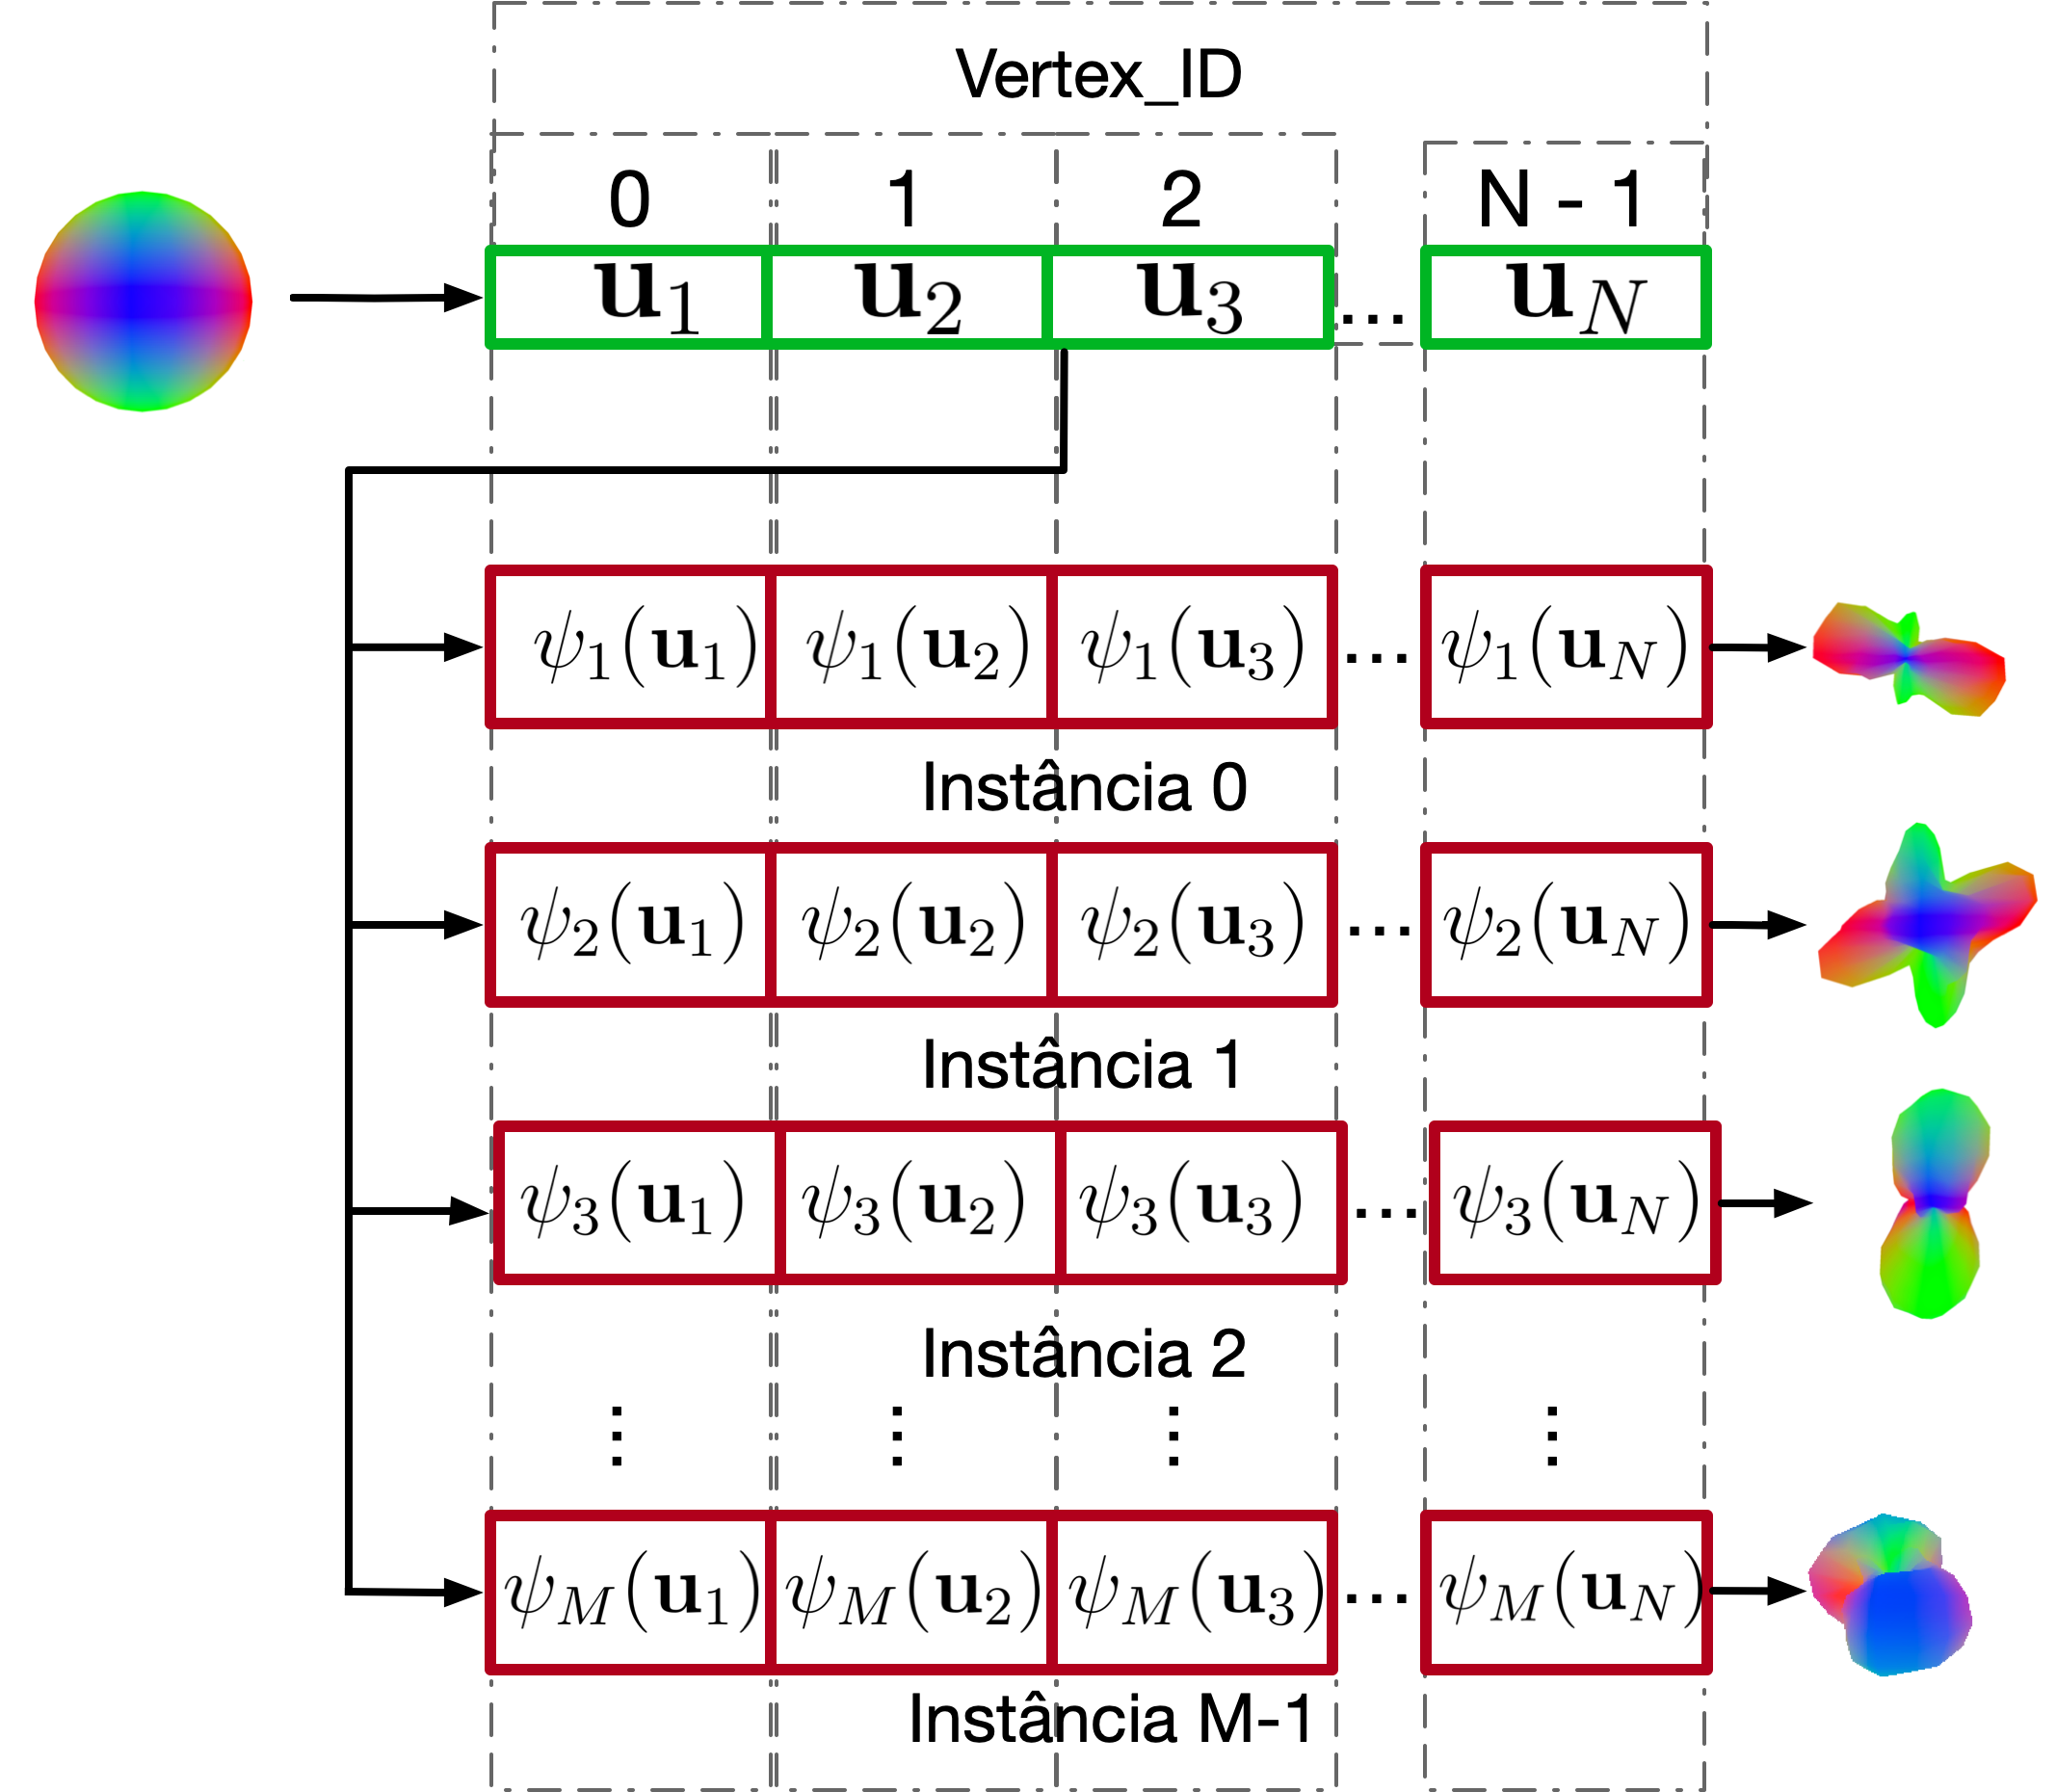
\includegraphics[width=1.0\linewidth, angle=0]{figs/Esquema_Glifo/GPU2GlifoGeneral.png}
    \caption{Ilustração da organização de dados na GPU da matriz de perfil de difusão (vermelho). Os vértices da malha esférica estão em verde. A cada instância, a customização do glifo se dá através da multiplicação do vértice da malha com o seu respectivo valor $\psi$, recuperado no \textit{vertex shader} através do seu índice de vértice para os P glifos a serem renderizados.}
    \label{fig::GPU2glifoGeneral}
   \hspace{1pt}
\end{figure}



\subsection{Otimização para ODFs simétricas}
\label{ssec::otimizacao}

Nesta subseção, mostramos uma adaptação da estrutura de dados descrita na subseção \ref{ssec::datastruct} para ODFs simétricas e uma estratégia para diminuir o seu respectivo tráfego de dados CPU-GPU pela metade.

Uma ODF é simétrica se $\psi(\mathbf{u}) = \psi (-\mathbf{u}) $ para todo $\mathbf{u}$ na esfera unitária. Esta simetria se aplica ao comportamento de difusão, o que torna esta seção aplicável para renderizar ODFs obtidas através de métodos HARDI.

Primeiramente, sugerimos o uso de uma malha esférica simétrica. Isso significa que se um ponto $P \in \Pi \implies -P \in \Pi$. Como exemplo, uma malha gerada por qualquer ordem de um icosaedro tesselado se encaixa nesse critério.

Em segundo lugar, sugerimos que a estrutura de dados da malha esférica simétrica escolhida seja organizada de forma que um ponto $P$ em um índice par seja seguido por $-P$. Esta malha esférica é enviada para a GPU da mesma forma indicada na subseção \ref{ssec::initializacao_glifo}.

Seguindo estas recomendações, a estrutura de dados dos pontos na esfera $[P_1, P_2, P_3, P_4, \dots, P_ {N-1}, P_N] $ torna-se $[P_1, -P_1, P_3, -P_3, \dots , P_ {N-1}, -P_ {N-1}]$ e seu respectivo conjunto $ \Upsilon$ se torna $[\mathbf{u}_1, - \mathbf{u}_1, \mathbf{u}_3, -\mathbf{u}_3, \dots, \mathbf{u}_{N-1}, - \mathbf{u}_{N-1}]$. Com os dados estruturados desta maneira, $\mathbf{\Psi}$ se torna:

\begin{equation}
\mathbf{\Psi} = 
\begingroup % keep the change local
\setlength\arraycolsep{2pt}
\begin{bmatrix} 
    \psi_1(\mathbf{u}_1) & \psi_1(-\mathbf{u}_1) & \cdots \psi_1(\mathbf{u}_{N-1}) & \psi_1(-\mathbf{u}_{N-1})  \\
    
     \psi_2(\mathbf{u}_1)& \psi_2(-\mathbf{u}_1) & \cdots \psi_2(\mathbf{u}_{N-1}) & \psi_2(-\mathbf{u}_{N-1}) \\

    \vdots & \vdots & \vdots & \vdots  \\
    
     \psi_M(\mathbf{u}_1)&\psi_M(-\mathbf{u}_1) & \cdots \psi_M(\mathbf{u}_{N-1}) & \psi_M(-\mathbf{u}_{N-1})
    
\end{bmatrix},
\endgroup
\end{equation}

onde cada (2k+1)-ésima coluna é a mesma (2k+2)-ésima ($0 \leq k < \frac{N}{2}$).

Portanto, definimos uma matriz $\mathbf{\Psi^h}_{Mx\frac{N}{2}}$ de tal forma que $\mathbf{\psi^h}_{ij} = \mathbf{\psi}_{i(2j-1)}$, descrita na expressão abaixo:

\begin{equation}
\label{eq::Psi_changed}
\mathbf{\Psi^h} = 
\begingroup % keep the change local
\setlength\arraycolsep{2pt}
\begin{bmatrix} 
    \psi_1(\mathbf{u}_1) & \psi_1(\mathbf{u}_3) & \cdots \psi_1(\mathbf{u}_{N-3}) & \psi_1(\mathbf{u}_{N-1})  \\
    
     \psi_2(\mathbf{u}_1)& \psi_2(\mathbf{u}_3) & \cdots \psi_2(\mathbf{u}_{N-3}) & \psi_2(\mathbf{u}_{N-1}) \\

    \vdots & \vdots & \vdots & \vdots  \\
    
     \psi_M(\mathbf{u}_1)&\psi_M(\mathbf{u}_3) & \cdots \psi_M(\mathbf{u}_{N-3}) & \psi_M(\mathbf{u}_{N-1})
    
\end{bmatrix}
\endgroup
\end{equation}


$\mathbf{\Psi^h}$ é enviado à GPU nas solicitações de desenho da mesma forma que $\mathbf{\Psi}$ descrito na subseção \ref{ssec::datastruct} e a diferença entre ambas está no \textit{lookup} na GPU. Na GPU, os vértices correspondentes ao 2k-ésimo e (2k+1)-ésimo Vértice\_ID na malha esférica da mesma instância têm o mesmo valor de lookup\footnote{Em OpenGL, a pesquisa é feita pelo comando texelFetch ($\mathbf{\Psi^h} $, ivec2 (gl\_InstanceID, gl \_VertexID/2), 0) [0]}, correspondendo à k-ésima coluna, que pode ser acessada adequadamente no \textit{vertex shader}.



\subsection{Visão geral dos \textit{shaders}}

\label{sssec::visao_shaders}

\subsubsection{Vertex Shader}
\begin{enumerate}
    \item Fazer o \textit{lookup} do valor de ODF que customiza o glifo e multiplicar o seu valor pelo seu respectivo vértice na esfera;
    \item transladar o glifo;
    \item escalonar e aplicar a transformação \textit{model-view-projection};
    \item computar a cor em função do vértice da malha esférica de acordo com a equação \ref{eq::cor_glifo} e enviar ao \textit{fragment shader}.
\end{enumerate}

\subsubsection{Fragment Shader}
\begin{enumerate}
    \item Definir a cor de saída como a cor rasterizada enviada pelo \textit{vertex shader}.
\end{enumerate}


%\section{Optimization}

%\todo[inline]{Is it not better to put together with other part of description?}





\section{Integração ao VMTK-Neuro}

No VMTK-Neuro, são computados a priori o conjunto de amostras de ODFs para uma determinada malha esférica e de matrizes de translação associados a cada um dos voxels.

Há um sistema de detecção de amostras do DWI aparentes na cena integrado ao VMTK-Neuro, tanto na renderização de fatias, quanto na renderização do volume em três dimensões.

Na renderização de fatias, a inferência dos \textit{pixels} aparentes na tela consiste na leitura dos índices do \textit{voxel} nas fatias coronais, axiais no qual os glifos são posicionados de acordo com a posição do seu respectivo \textit{pixel}.

Na renderização tridimensional, também há uma funcionalidade para detecção de amostras aparentes. A detecção é baseada em \textit{raycasting} computado sobre o volume na GPU, no qual foi proposto e implementado no VMTK-Neuro por \citeonline{raphael_dissertacao}. Cada uma das amostras é associado a uma matriz de translação pré-computada para o seu centro no 3D.

A partir de $M$ \textit{voxels} detectados em uma requisição de desenho, suas respectivas matrizes de posicionamento são copiadas e armazenadas como um vetor e enviadas à GPU. Da mesma maneira, a matriz $\mathbf{\Psi^h}$ é computada a partir das amostras detectadas e enviada à GPU, conforme mostrado na Figura \ref{fig::organizacao2GPU}.

\begin{figure}[ht]

%\subfigcapskip = -5pt
    \centering
    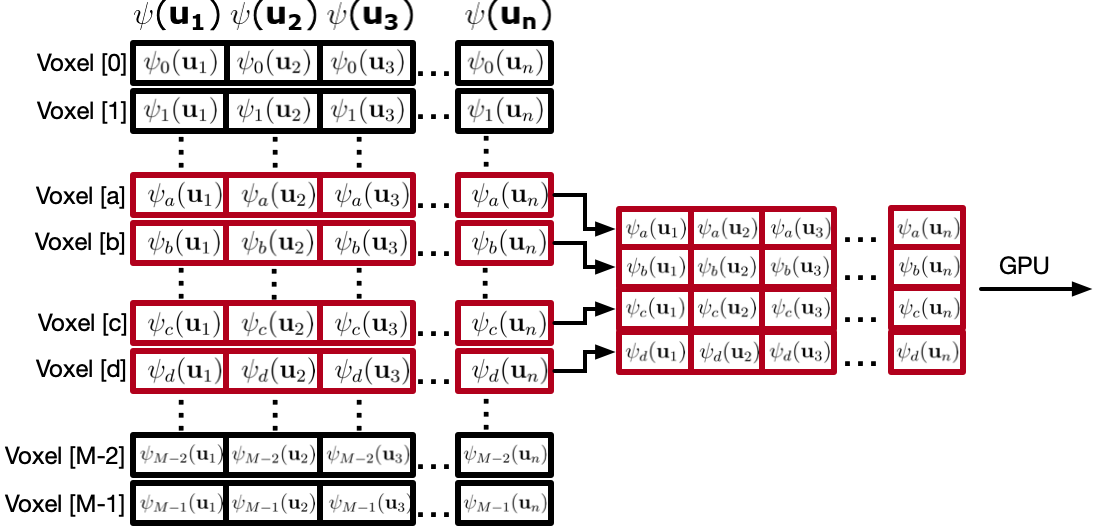
\includegraphics[width=1.0\linewidth, angle=0]{figs/Esquema_Glifo/organizacao2GPU.png}
    \caption{Ilustração da organização de dados de perfis de difusão antes do envio à GPU para um volume $V$ com $S$ \textit{voxels}. Cada perfil de difusão com $N$ amostras é pré-computado para todas os \textit{voxels} do volume. Em vermelho, estão os perfis de difusão de $M$ \textit{voxels} de ODF requisitados a serem desenhados, cujos índices são $d_1, d_2, \dots, d_M$, não necessariamente dispostos em sequência na memória. Estas amostras definem $\mathbf{\Psi^h}$ e são enviados à GPU.}
    \label{fig::organizacao2GPU}
   \hspace{1pt}
\end{figure}







Há elementos comuns a todos os glifos, que são enviados à GPU como variáveis uniformes. Estes elementos se referem a parâmetros de câmera na cena e a transformações relativas a orientação neurológica, que integram a matriz \textit{model-view-projection} e fator de escala.

As transformações relativas à orientação configuram a visualização de fatias para que fique compatível com um dos sistemas de orientação, que são a neurológica (LAS) e radiológica (RAS). O fator de escala é função do \textit{zoom} aplicado e dimensão do \textit{voxel}.





%O envio do conjunto de matriz de reposicionamento à GPU consiste no envio das coordenadas de translação como um atributo, que é único para cada malha esférica instanciada. Estes dados são armazenados \sout{por}\textcolor{red}{em} um \todo{Corresponde a qual objeto gráfico na GPU?}vetor, cujo índice se refere ao deslocamento da malha instanciada para seu respectiva posição.



%\subsection{\sout{Esquema de }Renderização na GPU}

%\todo[inline]{Para que o texto seja auto-contido, ou você referencia o trabalho do Raphael ou faz uma descrição completa para que o algoritmo seja reprodutível. Pois pelo que entendi, a sua proposta é uma variante da proposta do Raphael. É preciso deixar bem claro onde está a variação. O algoritmos é para GPU? Quantos passos são executados? Quais shaders?}

%A abordagem utilizada para renderização consiste em instanciações de uma malha esférica de N v centrada na origem e raio unitário, que é enviada à GPU uma única vez e sem repetição de vértices nos seus dados. A cada instância, a malha é transformada por duas classes de elementos: os elementos em comum a todos os \textit{voxels} e os particulares.

%O envio do conjunto de matriz de reposicionamento à GPU consiste no envio das coordenadas de translação como um atributo, que é único para cada malha esférica instanciada. Estes dados são armazenados \sout{por}\textcolor{red}{em} um \todo{Corresponde a qual objeto gráfico na GPU?}vetor, cujo índice se refere ao deslocamento da malha instanciada para seu respectiva posição.

%\todo[inline]{Suportar visualizações em LAS e RAS é uma demanda clínica e não por uma adequação ao VMTK ... }
%Os elementos comuns se referem às rotações e mudanças de escala. O fator de escala, que é função do \textit{zoom} aplicado e dimensão do \textit{voxel}, bem como o cômputo das transformações relativas à orientação, para que fiquem compatíveis com os sistemas de orientação neurológica (LAS) e radiológica (RAS) constam no VMTK-Neuro.% e sincronização com fatias bidimensionais.

%Há dois elementos particulares que customizam os glifos, cujos dados são enviados à GPU a cada \textit{frame} após os voxels aparentes na cena serem detectados. O primeiro é a translação para reposicionamento, que desloca a malha para o centro do seu respectivo \textit{voxel} e o segundo diz respeito às ODFs particulares a cada \textit{voxel}, que determina a forma do glifo através da multiplicação do vértice da malha associada à direção de difusão ao seu valor de ODF. %A implementação da matriz de reposicionamento foi algo direto, sendo uma adaptação do algoritmo dos glifos para DTI, pois o deslocamento é comum a todos os vértices instanciados. Já o mesmo não acontece com o mapa de ODFs.

%Para atingirmos o objetivo da interatividade, é necessário que o tráfego de dados CPU-GPU seja o mínimo possível e sem redundância. A maior parte deste tráfego se refere aos elementos particulares. Estes elementos são enviados à GPU a cada \textit{frame} de acordo com os \textit{voxels} visíveis detectados.

%\todo[inline]{Passou todos os dados para GPU como textura?}
%Os de ODF sim. Os de translação, não

%O envio do conjunto de matriz de reposicionamento para à GPU consiste na cópia de dados de deslocamento pré-computados para os \todo{Quais são os voxels detectados?}\textit{voxels} detectados. Estes dados são armazenados \sout{por}\textcolor{red}{em} um \todo{Corresponde a qual objeto gráfico na GPU?}vetor, cujo índice se refere ao deslocamento da malha instanciada para seu respectiva posição.

%O envio dos dados de ODF para GPU consiste na cópia dos dados referentes aos \textit{voxels} detectados de cada valor para cada perfil de difusão \todo{?}\textcolor{brown}{adotada consiste} na cópia dos dados de ODF para uma matriz pxn, onde p é a quantidade de \textit{voxels} detectados e n consiste na quantidade de amostras de ODF. A i-ésima linha da matriz se refere ao perfil de difusão do i-ésimo \textit{voxel} detectado, enquanto a j-ésima coluna se refere ao valor de difusão associado ao $\mathbf{u}_j$ para todos os \todo{Quais são os voxels detectados?}\textit{voxels} detectados. Esta matriz é enviada à GPU como uma textura 2D. A figura \ref{fig::organizacao2GPU} ilustra \todo{Não entendi ... a organização é dinâmica? Isso é muito custoso!}\textcolor{brown}{a organização dos dados para quando ocorre a detecção de quatro \textit{voxels}}.

%Teste



%\todo[inline]{Incluir os pseudocódigos de shaders não ajudaria o entendimento da ideia?}

%Na GPU, a malha esférica, copiada anteriormente e alocada em um \todo{VBO?}\textit{buffer}, é instanciada P vezes. Para a recuperação na GPU do perfil de difusão, é necessário que índice de vértice (\textit{gl\_VertexID}\footnotemark) da direção de cada um dos vértices correspondam à coluna do seu respectivo valor de ODF $\psi(\mathbf{u})$ da matriz de perfis de difusão. O acesso das linhas da matriz de perfis de difusão, correspondentes aos perfis de difusão de um \textit{voxel}acessível pelo índice de instância (\textit{gl\_InstanceID}\footnotemark[\value{footnote}]). Tendo os dados organizados desta maneira estabelecida, o acesso é feito no \textit{vertex shader} utilizando através da função \textit{texelFetch}\footnotemark[\value{footnote}] com os argumentos de acesso de linha e coluna através do par (\textit{gl\_VertexID}, \textit{gl\_InstanceID})\footnotemark[\value{footnote}]\footnotetext{Todos os comandos foram implementados em OpenGL com a linguagem para \textit{shader} GLSL.}. A forma de acesso na GPU da matriz de perfis de difusão como uma textura 2D é mostrada na figura \ref{fig::GPU2glifoGeneral}.


%\begin{figure}[h]
%%\subfigcapskip = -5pt
%    \centering
%    \includegraphics[width=.8\linewidth, %angle=0]{figs/Esquema_Glifo/GPU2Glifo%.png}
%    \caption{Ilustração da organização de %dados na GPU da matriz de perfil de %difusão (vermelho) enviados conforme %mostrado na figura %\ref{fig::organizacao2GPU}. Os %vértices da malha esférica estão em %verde. A cada instância, a %customização do glifo se dá através %da multiplicação do vértice da malha %com o seu respectivo valor $\psi$, %recuperado através do seu índice de %vértice.}
%    \label{fig::GPU2glifo}
%   \hspace{1pt}
%\end{figure}

\subsection{Resultados}

%\todo[inline]{Comentar que, para aproveitar as funcionalidades de interações gráficas disponíveis no VMTK-Neuro, o algoritmo foi integrado no VMTK-Neuro. Se puder, comentar os pontos de conexão.}

Na seção \ref{section::QBall_Glifos} do apêndice, seguem algumas imagens dos glifos derivados de ODFs integrados ao VMTK-Neuro. O volume é derivado da competição ISMRM \cite{TractometerTool}.

Medições em FPS em função da quantidade de glifos renderizadas foram feitas para malhas esféricas de 162, 642 e 2562 vértices e estão na figura \ref{fig::benchmark}, tanto na forma genérica de ODFs (figura \ref{fig::benchmark_full}), quanto na versão otimizada para ODFs simétricas (figura \ref{fig::benchmark_half}). Utilizamos paralelismo em CPU no processo de preparação dos dados a serem enviados à GPU.


O computador utilizado para o \textit{benchmark} foi um Macbook Pro Retina 13', com processador Intel Core i5 Dual-Core 2.7GHz, processador gráfico Intel Iris Graphics 6100 1536 MB e memória RAM de 8 GB 1867 MHz DDR3.

Os resultados mostram que o esquema pode ser utilizado de forma interativa. Pode-se renderizar milhares de glifos utilizando uma malha esférica com 162 vértices e centenas de glifos utilizando 2562 vértices em tempo interativo.

Há uma diferença relevante de performance na adaptação do esquema de renderização que toma vantagem da simetria de ODFs. Por exemplo, na performance da malha esférica de 642 vértices, sem otimização, a quantidade de glifos para renderizar em 60 FPS é menor que 2000, enquanto o esquema otimizado permite a renderização de um pouco mais de 4000 para mesma performance.

%Medições em FPS em função da quantidade de glifos renderizadas ao desempenho foram feitas para a quantidade de 197 e 422 vértices da malha esférica para diferentes quantidades de glifos renderizados e estão anotados nas tabelas \ref{tab::benchmark_glifos_197} e \ref{tab::benchmark_glifos_422}. O computador utilizado para o \textit{benchmark} foi um Macbook Pro Retina 13', com processador Intel Core i5 Dual-Core 2.7GHz, processador gráfico Intel Iris Graphics 6100 1536 MB e memória RAM de 8 GB 1867 MHz DDR3.

%Medições do tempo relativo ao desempenho foram feitas para a quantidade de 197 e 422 vértices da malha esférica para diferentes quantidades de glifos renderizados e estão anotados nas tabelas \ref{tab::benchmark_glifos_197} e \ref{tab::benchmark_glifos_422}. O computador utilizado para o \textit{benchmark} foi um Macbook Pro Retina 13', com processador Intel Core i5 Dual-Core 2.7GHz, processador gráfico Intel Iris Graphics 6100 1536 MB e memória RAM de 8 GB 1867 MHz DDR3.

%Os resultados estão também anotados como fração do limite de tempo de reação instantânea ($t_{max}$). Seja $t$ o intervalo de tempo entre a interação do usuário com um sistema e a sua respectiva resposta, mostrada de forma visual. O tempo $t_{max}$ é o limite máximo de $t$ em que o usuário tenha a percepção que o sistema reage instantaneamente as suas ações que, de acordo com \citeonline{nielsen1994}, é de 0,1s.

%\citeonline{nielsen1994} define o tempo de 0,1s 
%\todo{Não entendi ...}\textcolor{brown}{e que suas ações são a causa de que algo aconteça na tela }. 

%\todo[inline]{Percebeu oscilações nos tempos. A variação não é linear. Vamos ter que tentar entender por quê esta contra-intuitivo comportamento.}

%O resultados mostrados nas tabelas \ref{tab::benchmark_glifos_197} e \ref{tab::benchmark_glifos_422} mostram que centenas de glifos podem ser renderizados na faixa de centenas de microssegundos e unidades de milissegundos, o que possibilita a sua integração a esquemas de renderização mais complexos e custosos computacionalmente relacionados a volumes de difusão.

%\todo[inline]{O que é fração do limite máximo para interatividade?}
%\pagebreak

%Pode-se notar que em ambas as malhas esféricas utilizadas, a fração de tempo de execução é pequena para centenas







%A estratégia adotada para superar esse problema foi o  armazenamento dos dados de ODF dos \textit{voxels} detectados e o envio para GPU como uma textura 2D, onde é possível acessar os dados de ODF de acordo com índices de instância (relativo ao \textit{voxel}) e o índice de vértice (relativo à malha esférica instanciada na GPU), que requer uma organização específica para os dados enviados a cada \textit{frame}.

%O problema no valor de ODFs é que não há parâmetros em comum entre vértices da mesma esfera instanciada. A API OpenGL e a linguagem GLSL não oferecem formas diretas de se fazer alocação dinâmica de memória na GPU, em que disponibilize N*M valores de ODF para N \textit{voxels} aparentes na tela e uma malha esférica de M vértices.

%\todo[inline]{Como foi a estruturação na textura? Procurou explorar a coalescência/a sequência de acessos?}
%Evidentemente que há um mapeamento do domínio $[0,1]^2$, que é padrão numa unidade de textura, para a quantidade de instâncias e vértices que são processados.

%\todo[inline]{Há alguma explicação plausível para a queda de tempo na GPU entre 30 e 100 e entre 2000 e 5000?}

\begin{figure}[ht]
\centering
\captionsetup[subfloat]{farskip=0pt,nearskip=0pt}
    \subfloat[Esquema de renderização para ODFs genéricas ]{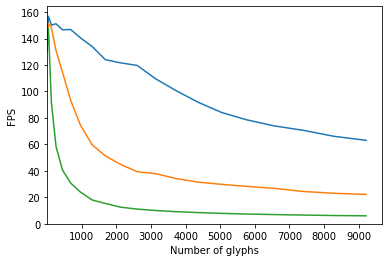
\includegraphics[width=.75\linewidth, angle=0]{figs/Esquema_Glifo/benchmark_full.png}
    \label{fig::benchmark_full}
    }
    %\hfill
    \\
    \subfloat[Esquema de renderização otimizado para ODFs simétricas ]{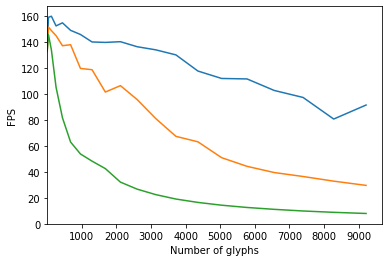
\includegraphics[width=.75\linewidth, angle=0]{figs/Esquema_Glifo/benchmark_half.png}
    \label{fig::benchmark_half}
    }
     \caption{FPS em função da quantidade de glifos renderizados. As curvas de cor azul, laranja e verde correspondem a medições feitas em malhas esféricas com 162, 642 e 2462 vértices, respectivamente. As malhas são geradas pelas subdivisões de $4^{a}$, $8^{a}$ e $16^{a}$ ordem do icosaedro}
    \label{fig::benchmark}
\end{figure}


%\begin{table}[H]
%\begin{tabular}{c|c|c|c|c}
%\textbf{\begin{tabular}[c]{@{}c@{}}Quantidade \\ de glifos\end{tabular}} & \textbf{\begin{tabular}[c]{@{}c@{}}Organização \\ e envio de \\ dados à GPU\\ ($\mu$s)\end{tabular}} & \textbf{\begin{tabular}[c]{@{}c@{}}Processamento\\ na GPU e \\ desenho ($\mu$s)\end{tabular}} & \textbf{\begin{tabular}[c]{@{}c@{}}Tempo de \\ execução\\ ($\mu$s)\end{tabular}} & \textbf{\begin{tabular}[c]{@{}c@{}}Fração do limite \\ máximo para\\ interatividade\end{tabular}} \\ \hline
%30                                                                       & 139.97                                                                                                 & 2097.00                                                              & 2236.97                                                                        & 2\%                                                                                               \\
%100                                                                      & 190.72                                                                                                 & 517.00                                                               & 707.72                                                                         & 1\%                                                                                               \\
%500                                                                      & 387.25                                                                                                 & 745.00                                                               & 1132.25                                                                        & 1\%                                                                                               \\
%2000                                                                     & 1352.93                                                                                                & 792.00                                                               & 2144.93                                                                        & 2\%                                                                                               \\
%5000                                                                     & 4768.94                                                                                                & 435.00                                                               & 5203.94                                                                        & 5\%                                                                                               \\
%10000                                                                    & 11886.44                                                                                               & 7798.00                                                              & 19684.44                                                                       & 20\%                                                                                             
%\end{tabular}
%\caption{\textit{Benchmark} de glifos representados por uma malha esférica de 197 vértices}
%\label{tab::benchmark_glifos_197}
%\end{table}


%\todo[inline]{Por quê a queda de tempo quando passa de 30 para 100? Alguma justificativa plausível?}
%\begin{table}[H]
%\begin{tabular}{c|c|c|c|c}
%\textbf{\begin{tabular}[c]{@{}c@{}}Quantidade \\ de glifos\end{tabular}} & \textbf{\begin{tabular}[c]{@{}c@{}}Organização \\ e envio de \\ dados à GPU\\ ($\mu$s)\end{tabular}} & \textbf{\begin{tabular}[c]{@{}c@{}}Processamento\\ na GPU e \\ desenho ($\mu$s)\end{tabular}} & \textbf{\begin{tabular}[c]{@{}c@{}}Tempo de \\ execução\\ ($\mu$s)\end{tabular}} & \textbf{\begin{tabular}[c]{@{}c@{}}Fração do limite \\ máximo para\\ interatividade\end{tabular}} \\ \hline
%30                                                                       & 270.40                                                                                               & 2174.00                                                              & 2444.40                                                                          & 2\%                                                                                               \\
%100                                                                      & 244.93                                                                                               & 447.00                                                               & 691.93                                                                           & 1\%                                                                                               \\
%500                                                                      & 724.67                                                                                               & 725.00                                                               & 1449.67                                                                          & 1\%                                                                                               \\
%2000                                                                     & 5439.72                                                                                              & 3384.00                                                              & 8823.72                                                                          & 9\%                                                                                               \\
%5000                                                                     & 13914.25                                                                                             & 5094.00                                                              & 19008.25                                                                         & 19\%                                                                                              \\
%10000                                                                    & 26841.13                                                                                             & 4773.00                                                              & 31614.13                                                                         & 32\%                                                                                             
%\end{tabular}
%\caption{\textit{Benchmark} de glifos representados por uma malha esférica de 422 vértices}
%\label{tab::benchmark_glifos_422}
%\end{table}





\chapter{Conclusões}

Neste trabalho foi abordamos a visualização de volumes DWI pelo método de imageamento para difusão Q-Ball, com o objetivo de integrá-lo ao ambiente multimodal em desenvolvimento pelo nosso grupo de pesquisa \cite{VMTKNeuro}, bem como desenvolver aplicações de visualização associadas. Adaptando muito do que já fora desenvolvido para o DTI, as aplicações desenvolvidas para o método consistem na estimação de ODFs via transformada de Funk-Radon, visualização em tempo interativo de ODFs em glifos e o desenvolvimento de um algoritmo de tractografia associado.

Objetivando prover um ambiente que permite a avaliação de ODFs, aproveitando as funcionalidades presentes no VMTK-Neuro para exploração de DWIs e MRI anatômicos, foi desenvolvido um esquema de renderização em tempo interativo que mapeia as ODFs em suas representações gráficas polares esféricas.

Com o objetivo de melhorar e tractografia baseada em DTI, foi implementado um protótipo de algoritmo de tractografia baseado em um conjunto de direções de métodos HARDI. !!(No trato corticoespinhal, no qual o DTI não consegue resolver).
Adicionalmente, a tractografia gera resultados em tempo interativo para o usuário, permitindo-o explorar livremente para diferentes parâmetros.

\section{Futuros trabalhos}

Na renderização de glifos, pode-se implementar o cômputo de vetores normais para serem usados na iluminação das superfícies, o que é algo comum na apresentação por glifos. Adicionalmente, podemos implementar as representações polares esféricas sugerida por \citeonline{hlawitschka2012} e/ou \citeonline{almsick2011} para fins de comparação de performance com a nossa abordagem.

Em tractografia, o próximo passo é a implementação do afiamento de ODFs, o que melhora extração de direções plausíveis de direções a serem usadas no \textit{tracking} de fibras \cite{fillard2011, SCHILLING2019194}.
\pagebreak
\chapter{Apêndice}


\section{Imagens de ODFs mapeadas em glifos renderizadas no VMTK-Neuro}

\label{section::QBall_Glifos}

\begin{figure}[H]
\label{fig::QBall_glifos_axial}
%\subfigcapskip = -5pt
    \centering
    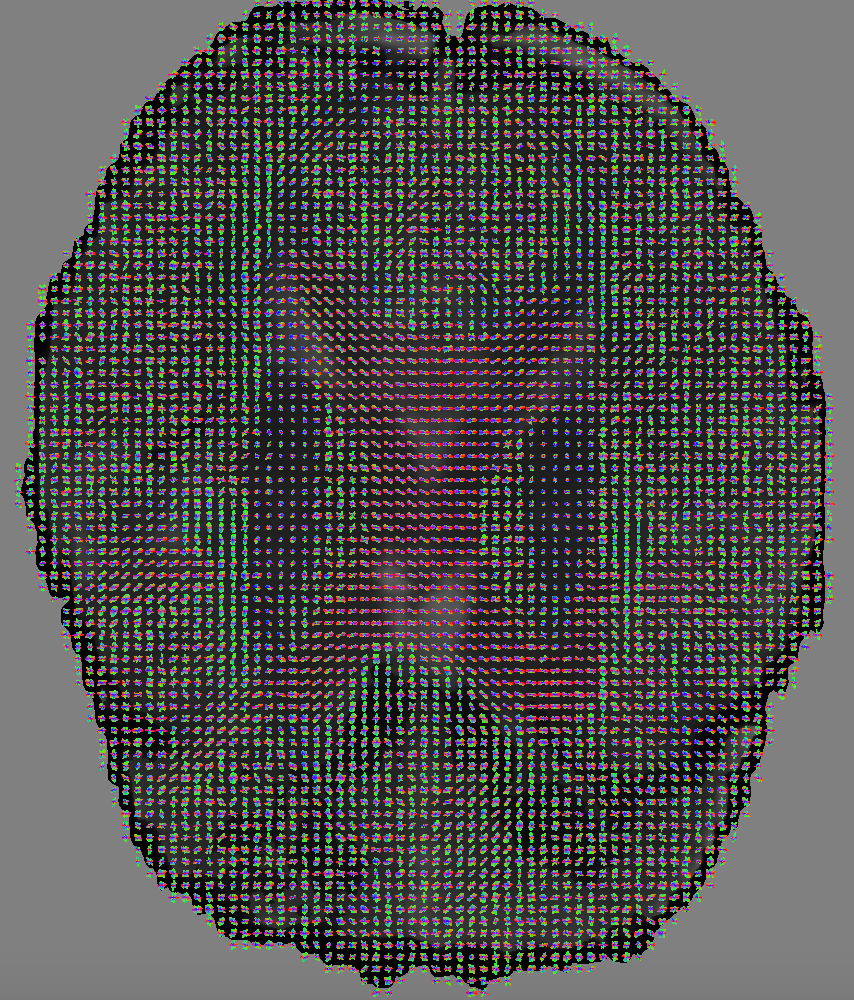
\includegraphics[width=1.0\linewidth, angle=0]{figs/Exemplos_QBall_visualizacao/Axial.png}
     \caption{Projeção Axial.}
 %   \hspace{1pt}
\end{figure}

\begin{figure}[H]
\label{fig::QBall_glifos_sagital}
%\subfigcapskip = -5pt
    \centering

    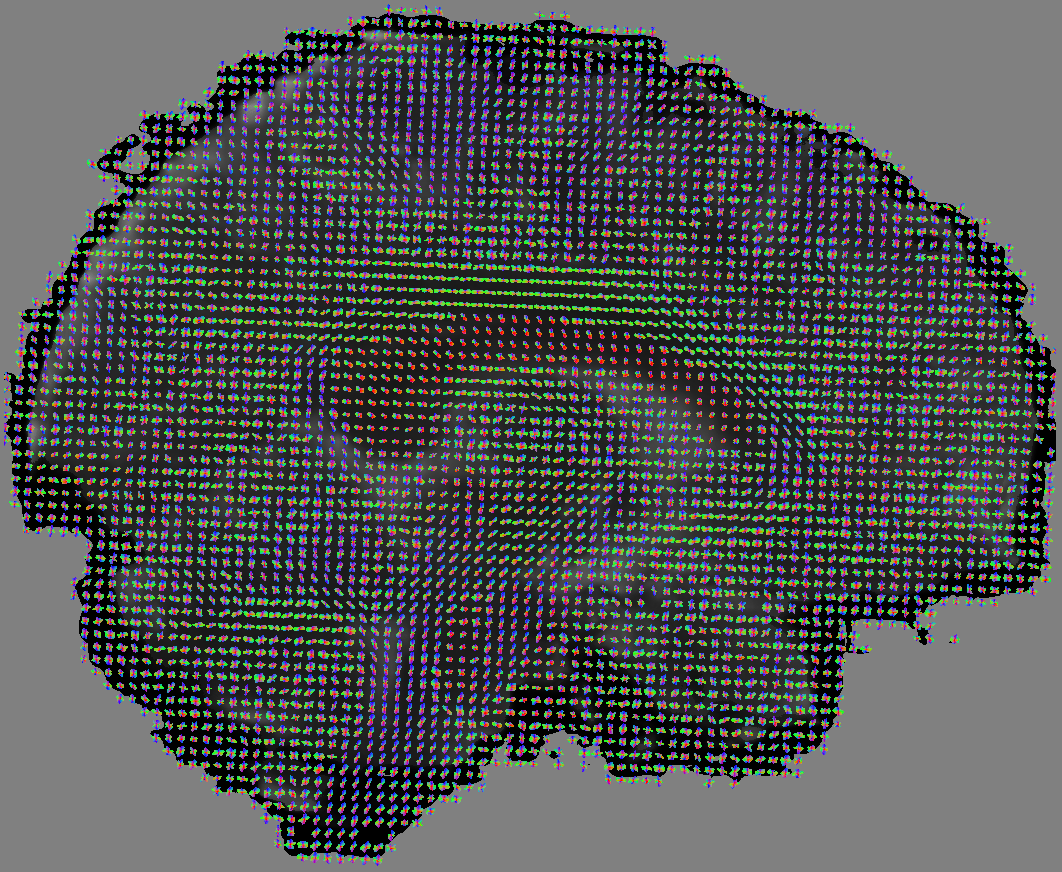
\includegraphics[width=.7\linewidth, angle=0]{figs/Exemplos_QBall_visualizacao/Sagital.png}
    \caption{Projeção Sagital.}
 %   \hspace{1pt}
\end{figure}

\begin{figure}[H]
\label{fig::QBall_glifos_coronal}
%\subfigcapskip = -5pt
    \centering

    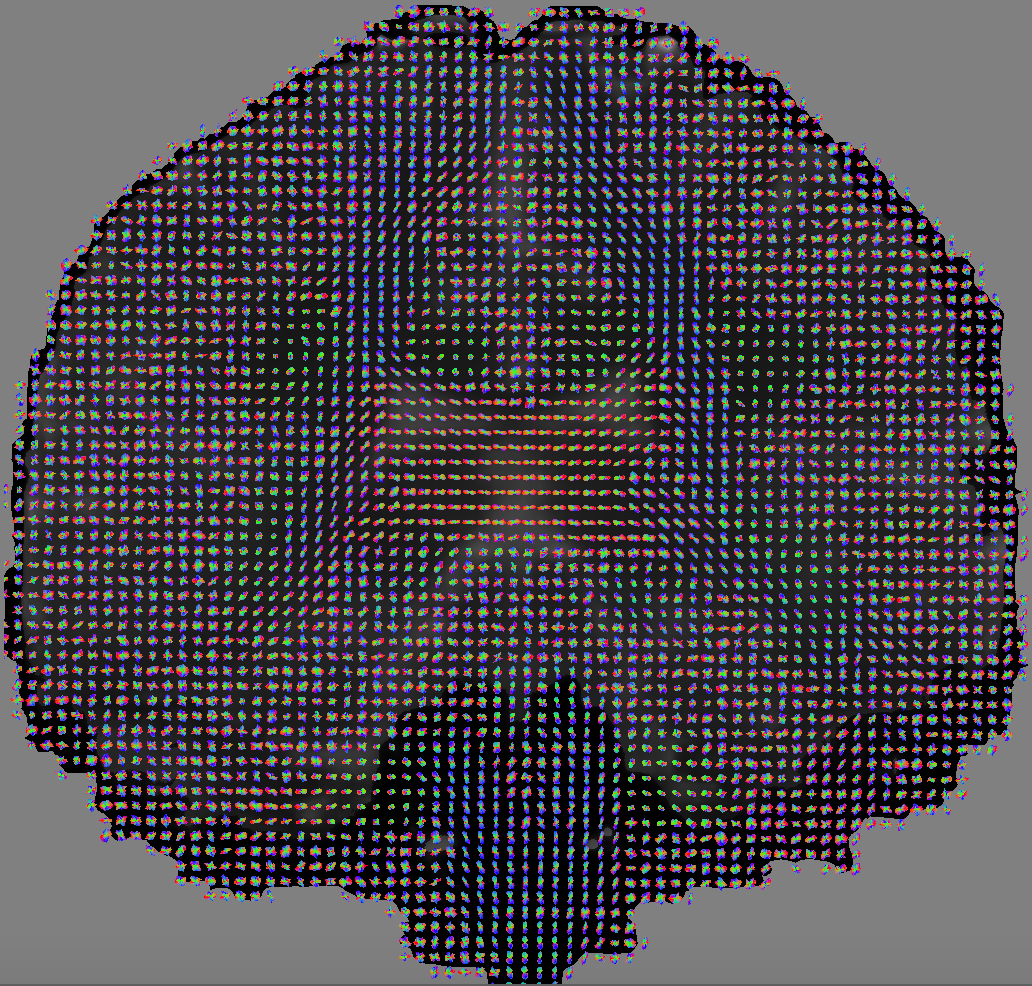
\includegraphics[width=0.7\linewidth, angle=0]{figs/Exemplos_QBall_visualizacao/Coronal.png}
    \caption{Projeção Coronal.}
 %   \hspace{1pt}
\end{figure}

\begin{figure}[H]
\label{fig::QBall_glifos_Coronal_CC_CS}
%\subfigcapskip = -5pt
    \centering
    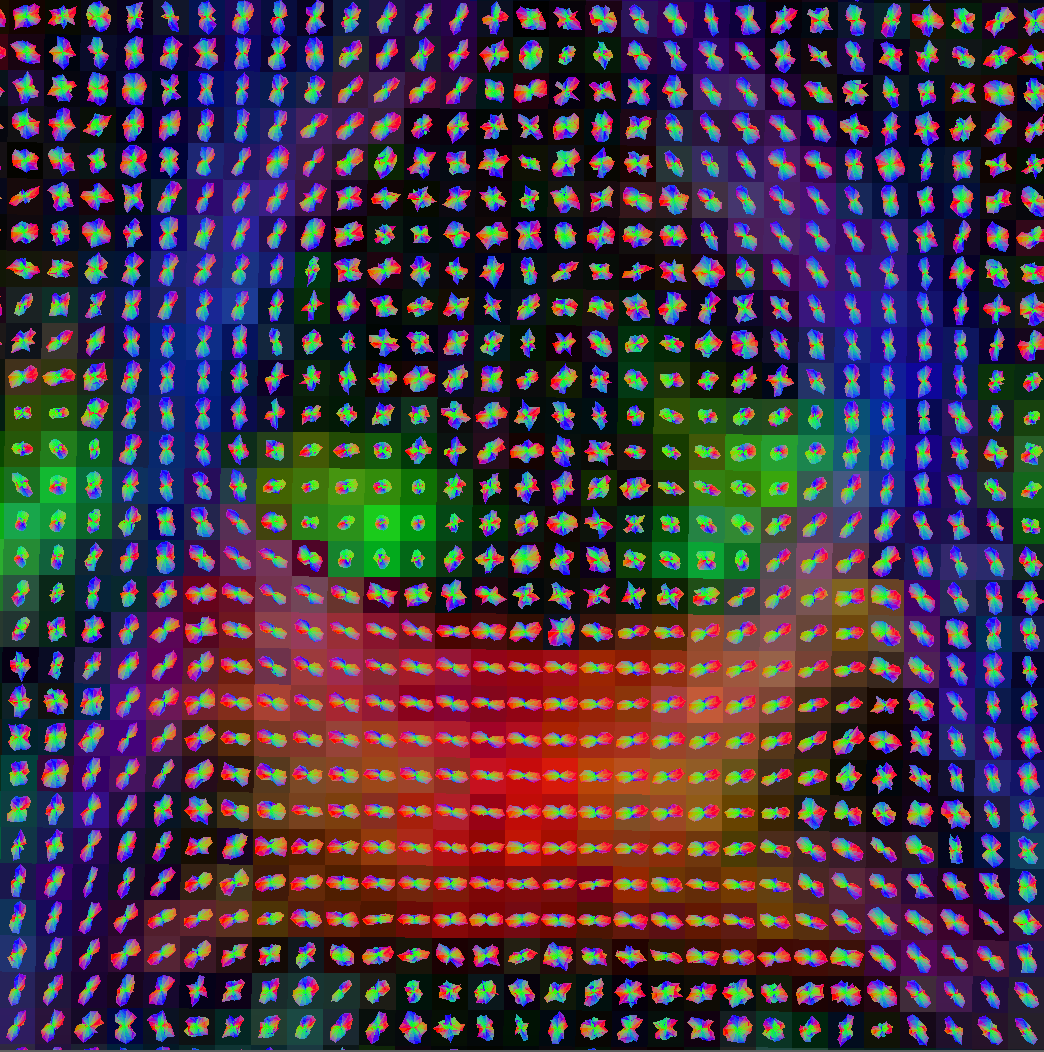
\includegraphics[width=.7\linewidth, angle=0]{figs/Exemplos_QBall_visualizacao/Coronal_Cruzamento_MapaFA.png}
    \caption{Projeção Coronal - Região de cruzamento de fibras. Glifos renderizado sobre mapa FA codificado por cores do DTI.}
 %   \hspace{1pt}
\end{figure}

\begin{figure}[H]
\label{fig::QBall_glifos_azul}
%\subfigcapskip = -5pt
    \centering

    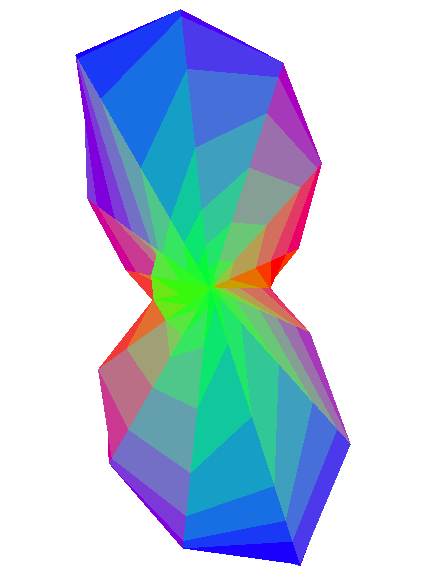
\includegraphics[width=.4\linewidth, angle=0]{figs/Exemplos_QBall_visualizacao/Glifo_Azul.png}
    \caption{Glifo referente a um voxel com direção de difusão predominantemente ascendente.}
 %   \hspace{1pt}
\end{figure}

\pagebreak


\section{\textit{Overplus} e problemas com o mapeamento do sinal de difusão em ODFs}
\label{ssec::problema_overplus}

Após um estudo que visou comparar ODFs geradas a partir de diferentes esquemas de amostragem de gradientes de ponderação de difusão, concluímos que a falta de uniformidade do conjunto de gradientes do \textit{Overplus} no domínio esférico compromete a interpolação de sinais de difusão no processo de cômputo do \textit{Q-Ball}. A figura \ref{fig::shell_Overplus_VS_ISMRM} mostra a distribuição no \textit{shell}\footnote{\textit{Shell} é um consiste em um conjunto definido em uma esfera.} das direções dos gradientes do \textit{Overplus}, em adição ao utilizado no volume ISMRM 2015.

\begin{figure}[ht]
\centering
\captionsetup[subfloat]{farskip=5pt,nearskip=0pt}
    %!!VER SE ISSO TA CERTO
    \subfloat[\textit{Overplus}.] {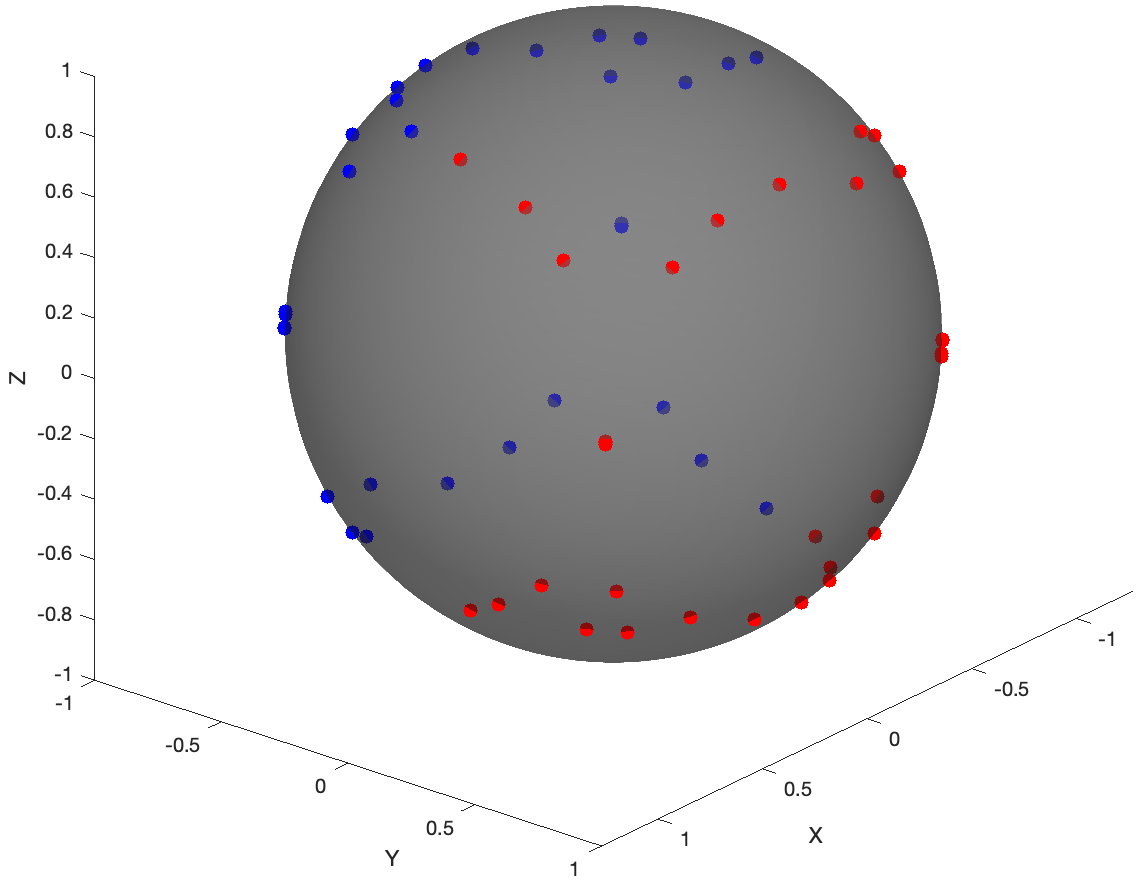
\includegraphics[width=.4\linewidth, angle=0]{figs/Overplus_VS_ISMRM/shell_overplus.png}}    
    \hfill
    \subfloat[Esquema utilizado no ISMRM.]{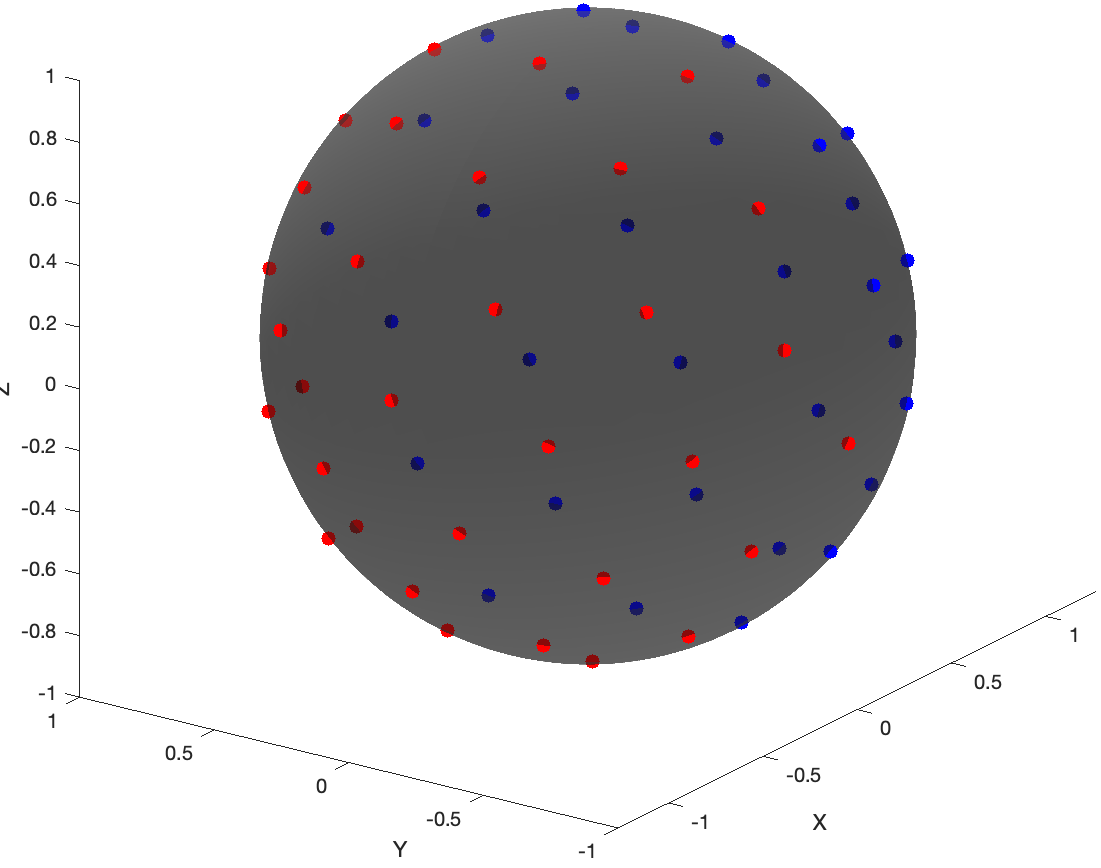
\includegraphics[width=.4\linewidth, angle=0]{figs/Overplus_VS_ISMRM/shell_ismrm.png}}
     \caption{Domínio esférico com pontos de amostragem referentes a direção de gradientes de difusão. Vermelho: direções de amostragem. Azul: sentido oposto da direção de amostragem.}
    %\hfill
    \label{fig::shell_Overplus_VS_ISMRM}
\end{figure}


Um bom conjunto de gradientes de codificação de difusão vinculada a um DWI não tem uma preferência direcional, as amostras no domínio esférico possuem uma boa invariância à orientação das estruturas do tecido ou coordenadas da máquina e a separação angular entre um par de pontos mais próximos é máxima e constante para todos os elementos \cite{cheng2018}. Um conjunto que segue essas propriedades estão distribuídos uniformemente sobre o \textit{shell}.

Há uma certa concordância na literatura de que uma uniformidade no domínio esférico em aquisições \textit{single shell}\footnote{Denomina-se aquisição \textit{single shell} como volumes de ressonância de difusão escaneados com apenas um valor b, além do b0.} é importante para uma boa reconstrução de ODFs. \citeonline{yeh2010} mencionam a importância da uniformidade além de propor uma métrica para aferir o seu grau. \citeonline{cheng2018} discorrem sobre formulações de esquemas de amostragem de gradientes de forma uniforme e mencionam as suas vantagens.

Como parte do processo de investigação dos resultados não esperados de ODFs gerados a partir dos volumes adquiridos através do protocolo \textit{Overplus}, foram escaneados para um mesmo indivíduo um volume com o conjunto de direções da competição ISMRM, o padrão, e um usando o protocolo \textit{Overplus} da Philips, em que todos possuem a mesma resolução angular de 32 direções. A análise feita consistiu na inspeção da forma dos glifos na região do corpo caloso que contém uma forte componente na direção mediolateral. A localização desta região se dá através do mapa FA codificado por cor gerado pelo DTI, em que não foi constatado nenhum problema nestes esquemas de aquisição.


Nesta inspeção, foi possível gerar glifos das ODFs razoáveis para o esquema de amostragem do ISMRM (Figura \ref{fig::Overplus_VS_ISMRM_b}), o que não aconteceu com o \textit{Overplus}, em que as ODFs ficaram totalmente descaracterizadas em comparação com os códigos de cores, conforme mostrado na Figura \ref{fig::Overplus_VS_ISMRM_a}.

\begin{figure}[ht]
\centering
\captionsetup[subfloat]{farskip=5pt,nearskip=0pt}
    
    \subfloat[\textit{Overplus}] {\label{fig::Overplus_VS_ISMRM_a} 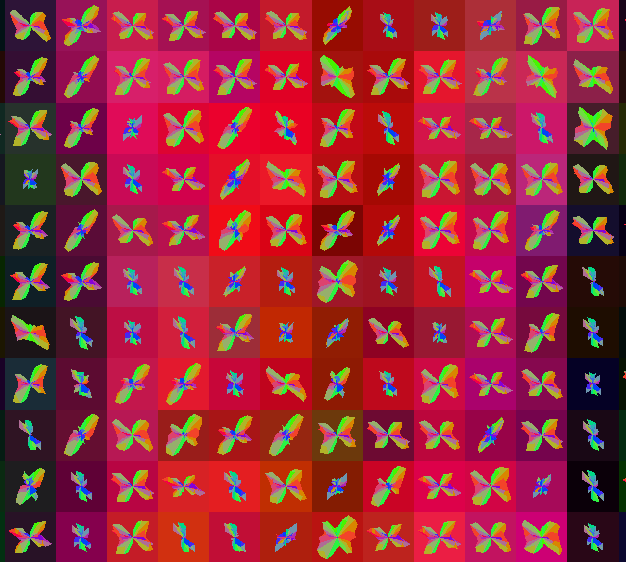
\includegraphics[width=.45\linewidth, angle=0, ]{figs/Overplus_VS_ISMRM/Overplus.png}}
    \hfill
    \subfloat[Esquema da competição ISMRM]{\label{fig::Overplus_VS_ISMRM_b} 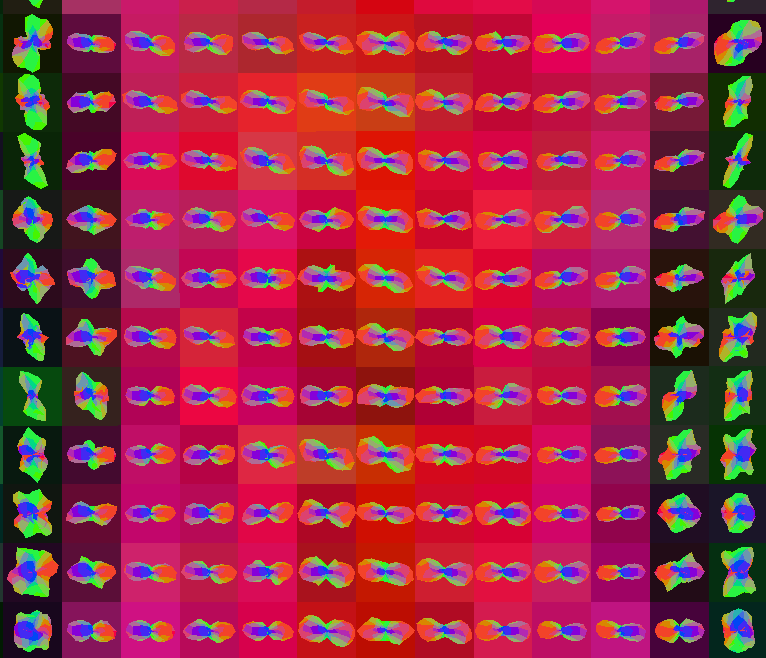
\includegraphics[width=.47\linewidth, angle=0]{figs/Overplus_VS_ISMRM/ISMRM.png}}
    %\hfill
    \caption{Glifos do Corpo Caloso - Mediolateral. Glifos de ODF sobre mapa FA codificado por cor do DTI.} %!!VER SE ISSO TA CERTO
    \label{fig::Overplus_VS_ISMRM}
\end{figure}
\pagebreak


%\bibliographystyle{}
\bibliography{references.bib}

% ----------------------------------------------------------
% Glossário
% ----------------------------------------------------------
%
% Consulte o manual da classe abntex2 para orientações sobre o glossário.
%
%\glossary

% ----------------------------------------------------------
% Apêndices
% ----------------------------------------------------------

% ---
% Inicia os apêndices
% ---
%\begin{apendicesenv}
%\end{apendicesenv}
% ---


% ----------------------------------------------------------
% Anexos
% ----------------------------------------------------------

% ---
% Inicia os anexos
% ---
\begin{anexosenv}
\end{anexosenv}

%---------------------------------------------------------------------
% INDICE REMISSIVO
%---------------------------------------------------------------------
%\phantompart
\printindex
%---------------------------------------------------------------------

\end{document}


